\documentclass[10pt,twocolumn]{article}

% Line spacing
\renewcommand{\baselinestretch}{1.05}
\widowpenalty=10000
\clubpenalty=10000
\hyphenpenalty=300
\tolerance=1000

% Packages
\usepackage[T1]{fontenc}
\usepackage{mathpazo}
\usepackage[scaled=0.9]{helvet}
\usepackage{courier}
\usepackage{microtype}
\usepackage{graphicx}
\usepackage{dblfloatfix}
\usepackage{adjustbox}
\usepackage{amsmath}
\usepackage{mathtools}
\usepackage{amsfonts}
\providecommand{\qed}{\hfill$\square$}
\usepackage{pifont}
\usepackage{amssymb}
\usepackage{booktabs}
\usepackage{tabularx}
\usepackage[table]{xcolor}
\usepackage{listings}
\definecolor{codebg}{HTML}{F8F9FA}
\definecolor{codeframe}{HTML}{E9ECEF}
\lstdefinestyle{elegant}{
    backgroundcolor=\color{codebg},
    basicstyle=\ttfamily\footnotesize,
    breaklines=true,
    frame=single,
    rulecolor=\color{codeframe},
    numbers=none,
    keywordstyle=\color{harvardcrimson}\bfseries,
    commentstyle=\color{codegreen}\itshape,
    stringstyle=\color{blue},
    xleftmargin=1em,
    xrightmargin=1em,
    framexleftmargin=0.5em,
    framexrightmargin=0.5em,
    framextopmargin=0.5em,
    framexbottommargin=0.5em,
    captionpos=b,
    aboveskip=1.5em,
    belowskip=1.5em
}
\lstset{style=elegant}
\PassOptionsToPackage{hyphens,spaces,obeyspaces}{url}
\usepackage[round,authoryear]{natbib}
\bibliographystyle{plainnat}
\usepackage{hyperref}
\usepackage{cleveref}
\usepackage{enumitem}
\usepackage{titlesec}
\usepackage{subcaption}
\usepackage{float}
\usepackage{placeins}
\usepackage{balance}
\usepackage[most]{tcolorbox}

% Caption styling
\usepackage{caption}
\captionsetup{font=small, labelfont=bf, labelsep=period, justification=justified, singlelinecheck=false, skip=8pt, belowskip=0pt}
\captionsetup[table]{position=top}
\setlength{\textfloatsep}{10pt plus 2pt minus 2pt}

% Section titles
\titleformat{\section}
  {\normalfont\Large\bfseries\raggedright}{\thesection}{0.75em}{}
\titleformat{\subsection}
  {\normalfont\large\bfseries\raggedright}{\thesubsection}{0.65em}{}
\titleformat{\subsubsection}
  {\normalfont\fontsize{11}{13}\selectfont\bfseries\raggedright}{\thesubsubsection}{0.5em}{}
\titlespacing*{\section}{0pt}{0.8\baselineskip}{0.5\baselineskip}
\titlespacing*{\subsection}{0pt}{0.6\baselineskip}{0.4\baselineskip}
\titlespacing*{\subsubsection}{0pt}{0.5\baselineskip}{0.3\baselineskip}

% Page geometry
\usepackage[letterpaper, margin=1in]{geometry}
\usepackage{etoolbox}
\makeatletter
\patchcmd{\@maketitle}{\vskip 2em}{\vskip 0pt}{}{}
\makeatother

% Pin full-width floats to top
\makeatletter
\setlength{\@dblfptop}{0pt}
\setlength{\@dblfpbot}{0pt plus 1fil}
\makeatother

% Colors
\definecolor{harvardcrimson}{HTML}{A31F34}
\definecolor{codegreen}{HTML}{2D7A2D}
\definecolor{codegray}{HTML}{555555}
\definecolor{lightgray}{HTML}{F5F5F5}
\definecolor{napkinbg}{HTML}{FFF8E1}
\definecolor{napkinframe}{HTML}{C87B2A}
\definecolor{errorbg}{HTML}{FDE8E8}
\definecolor{errorframe}{HTML}{C44444}

\hypersetup{
  colorlinks=true,
  linkcolor=harvardcrimson,
  citecolor=blue,
  urlcolor=blue
}
\newcommand{\hrefurl}[2]{\href{#1}{\textcolor{blue}{#2}}}

% Napkin-math callout box (pedagogical worked examples)
\newtcolorbox{napkinmath}[1]{%
  enhanced,
  breakable,
  sharp corners,
  boxrule=0.8pt,
  colframe=napkinframe,
  colback=napkinbg,
  colbacktitle=napkinframe!15,
  coltitle=black!80,
  fonttitle=\small\bfseries\sffamily,
  title={Napkin Math: #1},
  toptitle=0.5ex,
  bottomtitle=0.5ex,
  left=0.8em,
  right=0.8em,
  top=0.6em,
  bottom=0.4em,
  before skip=\baselineskip,
  after skip=0.5\baselineskip,
  fontupper=\small,
}

% Error-case callout box (pedagogical failure examples)
\newtcolorbox{errorcase}[1]{%
  enhanced,
  breakable,
  sharp corners,
  boxrule=0.8pt,
  colframe=errorframe,
  colback=errorbg,
  colbacktitle=errorframe!15,
  coltitle=black!80,
  fonttitle=\small\bfseries\sffamily,
  title={Failure Case: #1},
  toptitle=0.5ex,
  bottomtitle=0.5ex,
  left=0.8em,
  right=0.8em,
  top=0.6em,
  bottom=0.4em,
  before skip=\baselineskip,
  after skip=0.5\baselineskip,
  fontupper=\small,
}

% Exercise callout box (structured classroom exercises)
\newtcolorbox{exercise}[1]{%
  enhanced,
  breakable,
  sharp corners,
  boxrule=0.8pt,
  colframe=harvardcrimson!70!black,
  colback=harvardcrimson!3,
  colbacktitle=harvardcrimson!12,
  coltitle=black!80,
  fonttitle=\small\bfseries\sffamily,
  title={Exercise: #1},
  toptitle=0.5ex,
  bottomtitle=0.5ex,
  left=0.8em,
  right=0.8em,
  top=0.6em,
  bottom=0.4em,
  before skip=\baselineskip,
  after skip=0.5\baselineskip,
  fontupper=\small,
}

% Table body text
\newcommand{\tablebody}{\footnotesize}

% ============================================================================
% Computed Constants — single source of truth for inline math
% ============================================================================
\usepackage{pgfmath}
\newcommand{\cval}[1]{\pgfmathprintnumber[fixed, precision=1, 1000 sep={\,}]{#1}}
\newcommand{\cvalint}[1]{\pgfmathprintnumber[fixed, precision=0, 1000 sep={\,}]{#1}}

%  ( Base hardware constants (H100 SXM datasheets) )
\pgfmathsetmacro{\HhPeakTFLOPS}{989}
\pgfmathsetmacro{\HhBWTBs}{3.35}
\pgfmathsetmacro{\HhHBMGB}{80}
\pgfmathsetmacro{\NVLinkBWGBs}{900}
\pgfmathsetmacro{\IBBWGBs}{50}
\pgfmathsetmacro{\SRAMperSMKB}{228}

%  ( Derived: Roofline )
\pgfmathsetmacro{\HhRidgePoint}{\HhPeakTFLOPS / \HhBWTBs}

%  ( Derived: Attention walkthrough )
\pgfmathsetmacro{\SeqLen}{8192}
\pgfmathsetmacro{\HeadDim}{128}
\pgfmathsetmacro{\NumHeads}{32}
\newcommand{\AttnIntermMB}{128}       % 8192^2 * 2 / 1048576
\newcommand{\AttnTotalGB}{4}          % 128 * 32 / 1024
\pgfmathsetmacro{\TileSize}{256}
\newcommand{\TileKB}{128}  % 256*256*2/1024

%  ( Model constants )
\pgfmathsetmacro{\LLaMAParams}{70}
\pgfmathsetmacro{\LLaMAWeightsGB}{140}

%  ( Derived: ZeRO )
\pgfmathsetmacro{\ZeROMemGB}{1120}  % 140+140+840
\pgfmathsetmacro{\ZeROMinDevices}{14}  % ceil(1120/80)

%  ( Derived: MoE )
\pgfmathsetmacro{\MoEExperts}{16}
\pgfmathsetmacro{\MoEExpertGB}{8}
\pgfmathsetmacro{\MoETotalGB}{128}
\pgfmathsetmacro{\NVLinkIBgap}{\NVLinkBWGBs / \IBBWGBs}

% --- Edge-device constants (Apple M4 Pro, representative unified-memory SoC) ---
\pgfmathsetmacro{\EdgeRAMGB}{36}
\pgfmathsetmacro{\EdgeBWGBs}{273}
\pgfmathsetmacro{\EdgeTFLOPS}{53}
\newcommand{\EdgeCtxTokens}{1\,000\,000}
\newcommand{\EdgeCtxTokensRaw}{1000000}
\pgfmathsetmacro{\EdgeKVPerTokenMB}{0.5}
\newcommand{\EdgeKVTotalGB}{488}  % 0.5 MiB * 1M tokens / 1024 = 488 GiB

%  ( Tensor parallelism constants )
\pgfmathsetmacro{\TPdevices}{8}
\pgfmathsetmacro{\TPweightsPerDevice}{17.5}  % 140/8

\begin{document}

\title{
  \textbf{A Design Grammar for ML Systems}\\[0.3em]
  {\large Primitives, Constraints, and Rewrite Rules}
}

\author{
  Vijay Janapa Reddi\\
  Harvard University
}

\date{\hrefurl{https://mlsysbook.ai}{mlsysbook.ai}}

\maketitle
\begingroup
\renewcommand{\thefootnote}{}%
\footnotetext{Part of the \emph{Machine Learning Systems} book ecosystem. Open-source tools: \url{https://mlsysbook.ai}.}%
\endgroup

\begin{abstract}
The rapid evolution of machine learning systems has produced a catalog of isolated techniques, from FlashAttention and ZeRO to PagedAttention and Megatron-LM, that obscures the field's underlying structure. We present a \emph{design grammar for ML systems}: a formal tuple $G=(P,O,T,C,R)$ consisting of primitive vocabulary, composition operators, typing rules, cost semantics, and rewrite rules. The grammar separates the stable building blocks of ML systems from the faster-moving systems built from them. Each primitive is admitted via an irreducibility criterion on performance cost; each rewrite rule records the constraints it relieves, the semantics it preserves, and the preconditions under which it applies. We validate the grammar through five end-to-end walkthroughs that derive state-of-the-art systems from first principles using hardware constraints and napkin math, including a dead-end analysis on an open million-token edge-deployment case that prunes wrong candidate rewrites before engineering effort is spent. We formalize composition through \emph{System Assembly Notation}, with Roofline-grounded cost semantics and three first-order performance bounds. The result is a teaching and design framework that turns ML systems from a memorized catalog of branded techniques into a derivable, physically grounded grammar of design choices.
\end{abstract}

\begin{figure*}[t!]
  \centering
  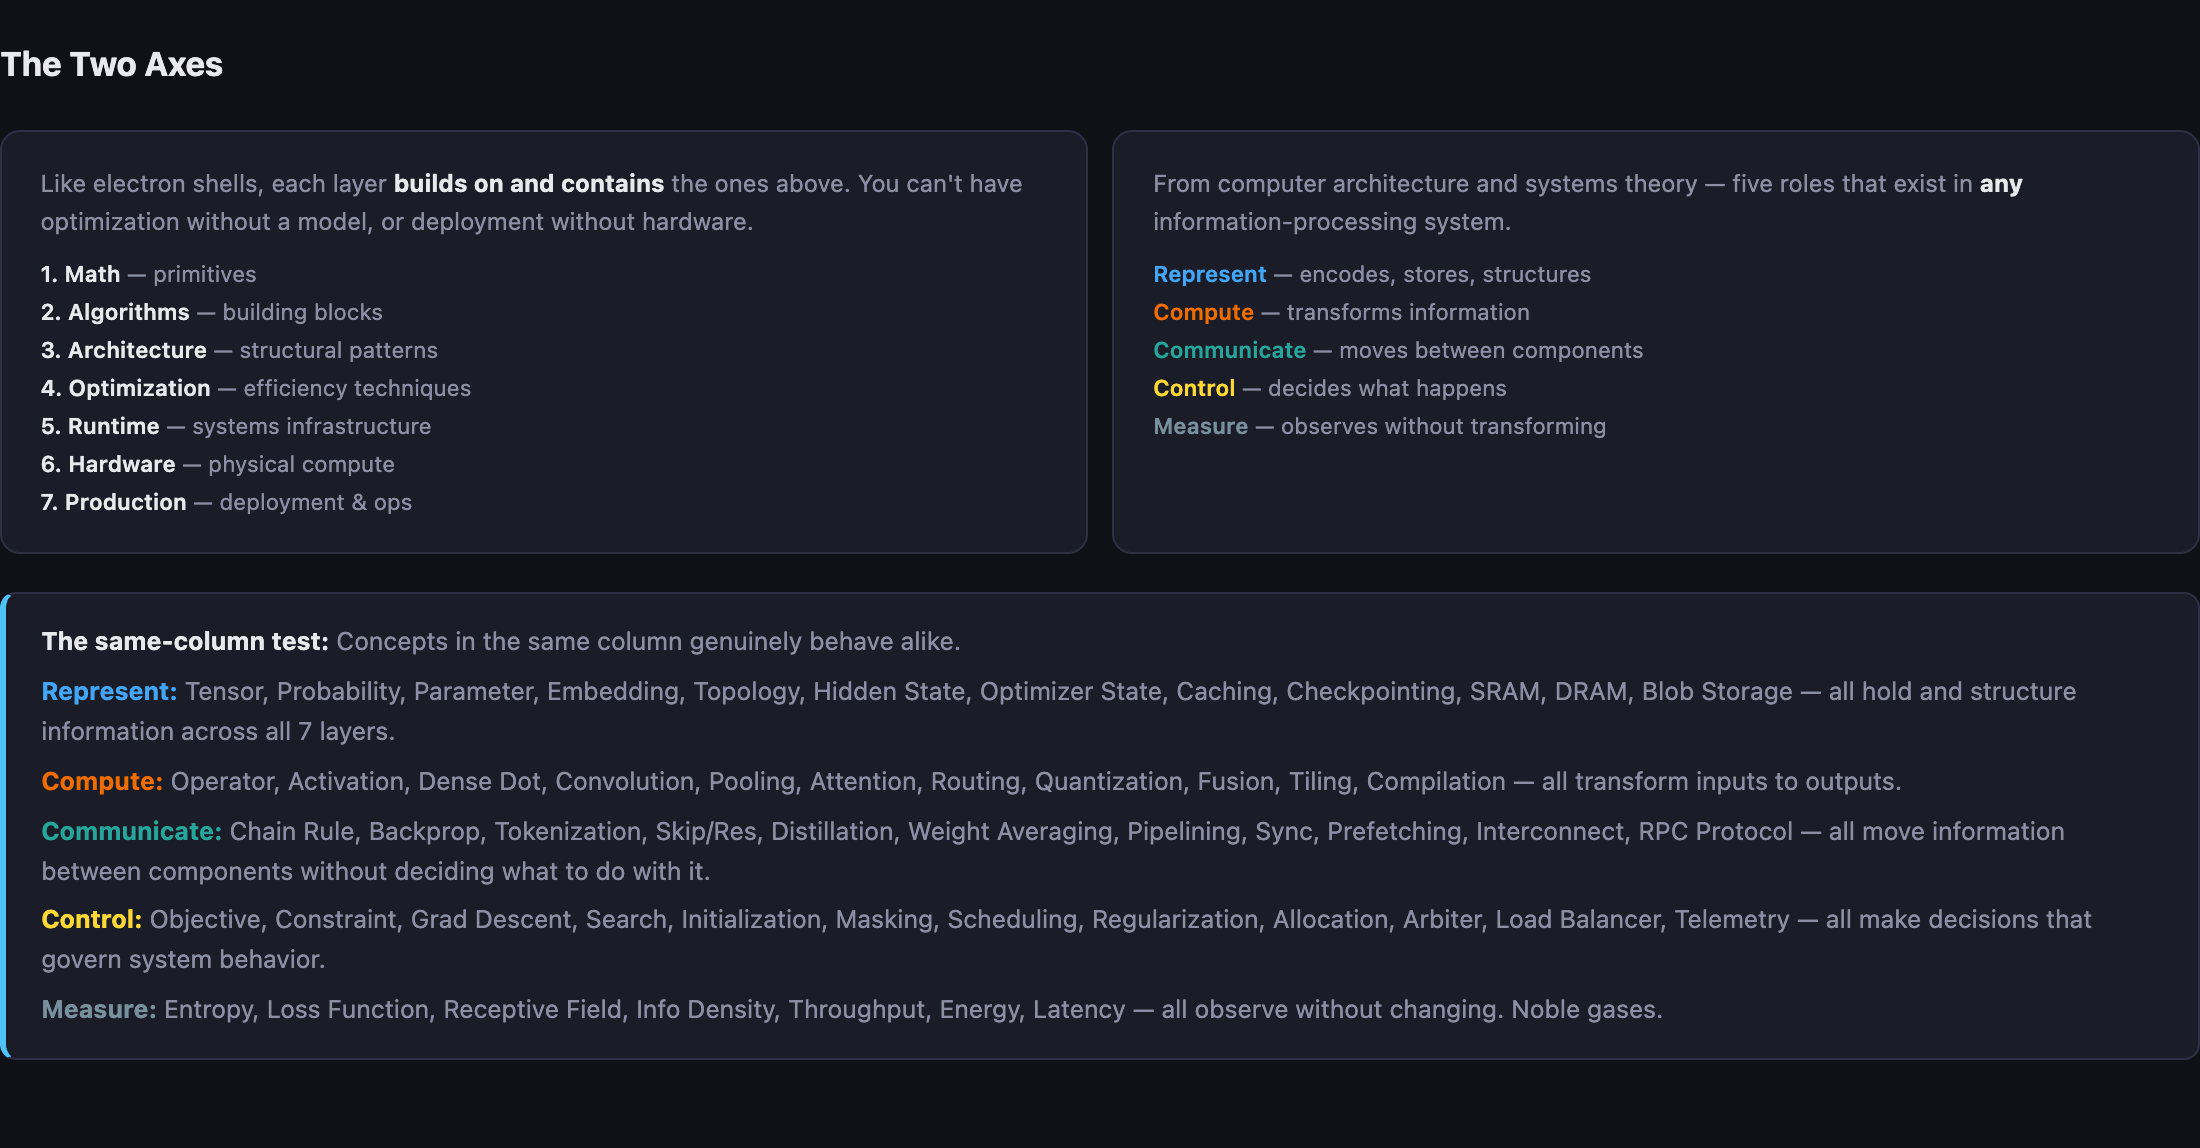
\includegraphics[width=\textwidth]{figures/primitive_catalog.pdf}
  \caption{\textbf{The primitive vocabulary of the ML Systems Design Grammar.} The catalog organizes 90 primitives along eight abstraction layers (Data through Production) and five information-processing roles (Represent through Measure). Each primitive satisfies a formal irreducibility criterion (\Cref{sec:irreducibility}): its performance cost cannot be modeled at its own layer without lowering to the layer below. The catalog supplies the vocabulary $P$; the operators, typing rules, cost semantics, and rewrite rules (\Cref{sec:composition,sec:resolution}) explain which compositions are valid and which rewrites are triggered when capacity, bandwidth, latency, utilization, or reliability constraints bind. Color encodes role: blue for Represent, orange for Compute, teal for Communicate, yellow for Control, gray for Measure.}
  \label{fig:primitive-catalog}
\end{figure*}

% ============================================================================
\section{Introduction}
\label{sec:intro}

The design of modern machine learning systems is defined by a fundamental tension: the growing gap between high-level algorithmic intent and the unforgiving reality of physical hardware. Consider a researcher writing \texttt{y = softmax(QK\textsuperscript{T}/$\sqrt{d}$)V}. While the mathematical intent is simply "attention," physical execution must materialize matrices in HBM, stream them at ${\sim}$\cval{\HhBWTBs}\,TB/s, and execute $O(n^2 d)$ multiply-accumulates on tensor cores. As sequence lengths grow, the quadratic memory footprint quickly exceeds the \cvalint{\HhHBMGB}\,GB capacity of an H100 GPU, making a rewrite such as tiling or fusion necessary.

The same pattern recurs across the field: a physical constraint binds, and the system must be rewritten without changing model semantics. FlashAttention for attention memory, ZeRO for distributed training memory, PagedAttention for serving fragmentation, and Megatron-LM for tensor parallelism all follow this shape. Yet the field is still often taught as a disconnected catalog of branded techniques, each presented as a standalone invention rather than a response to the same small family of physical constraints.

This paper makes that recurring structure explicit as the \emph{ML Systems Design Grammar}. Formally, we write the grammar as
\begin{equation}
\label{eq:grammar}
G = (P, O, T, C, R).
\end{equation}
$P$ is the primitive vocabulary shown in \Cref{fig:primitive-catalog}: 90 primitives spanning eight abstraction layers and five information-processing roles. $O$ defines the spatial, temporal, and dependency operators in System Assembly Notation. $T$ specifies which assemblies are well formed. $C$ evaluates an assembly against physical constraints. $R$ maps a violating assembly $M \mid_C$ to a candidate assembly $M'$ using behavior-preserving rewrites such as tiling, fusion, sharding, caching, quantization, scheduling, and replication.

The grammar is meant to be used constructively. A designer writes the naive assembly, estimates the first binding constraint, applies the smallest matching rewrite, recomputes the cost, and repeats. The primitive catalog is useful, but only as the vocabulary $P$ of the grammar.

What makes this a grammar is the combination of vocabulary, operators, typing rules, cost semantics, and rewrite rules. That combination lets FlashAttention, ZeRO, PagedAttention, and Megatron-LM be read as systematic recompositions of stable building blocks under changing physical constraints. A taxonomy labels objects; a grammar specifies legal compositions, compositional costs, and admissible transformations.

The intended use is both pedagogical and architectural. In teaching, the grammar turns named techniques into derivations; the walkthroughs (\Cref{sec:walkthrough}) and worked napkin-math examples (\Cref{sec:teaching}) provide a curriculum backbone that survives the churn of system names. For graduate students and researchers, it gives a way to read recent ML systems papers as instances of recurring constraint responses. For system architects, the same notation provides a structured whiteboard language for narrowing the rewrite space at design time rather than after an incident.

The scope is architectural, not operational. This paper is not a runtime, compiler, or programming language; it is a notation and cost model for order-of-magnitude design reasoning. Within deterministic, steady-state designs on single nodes or small homogeneous clusters, the grammar is meant to identify which constraint binds and what class of rewrite can relieve it (\Cref{sec:composition}). It does not replace cycle-accurate simulators, compiler IRs, or hardware profilers. System Assembly Notation is analogous to big-$O$ for algorithms: useful for the first design decision, not for generating machine code. Beyond a single node, constraints become probabilistic, and the constraint operator generalizes to $M \mid_{C,\, p > \theta}$ (\Cref{sec:probabilistic}).

The closest prior frameworks each cover part of this picture. The Roofline model \citep{williams2009} characterizes individual kernels; the Berkeley 13 Dwarfs \citep{asanovic2006landscape} classifies parallel motifs; Sze, Chen, Yang, and Emer's \emph{Efficient Processing of Deep Neural Networks} \citep{sze2020} catalogs accelerator dataflows and memory hierarchies; and MLSysIM \citep{reddi2026mlsysim} formalizes ``Systems Walls'' as hard physical bounds. None combines a primitive vocabulary with composition operators, cost semantics, and rewrite rules that turn a constraint violation into candidate system transformations. That is the gap this paper fills.

This constraint-driven framing does not deny historical contingency. Hooker's ``Hardware Lottery'' \citep{hooker2020hardware} argues that adopted architectures are often historical accidents of which ideas happened to fit which hardware at which time. We agree that hardware history shapes the field. The claim here is conditional: once a hardware target and workload are fixed, physical limits make some software rewrites useful, make others irrelevant, and rule out many outright. The design grammar gives that conditional reasoning a vocabulary and a calculus.

\paragraph{Contributions.}

\begin{enumerate}[nosep, leftmargin=*, label=\textbf{C\arabic*.}]
\item \textbf{The ML Systems Design Grammar.} A framework $G=(P,O,T,C,R)$ with a vocabulary of 90 primitives, composition operators, typing and validity rules, physical cost semantics, and rewrite rules for deriving feasible assemblies. This makes the primitive catalog one component of a larger grammar rather than a standalone taxonomy (\Cref{sec:primitive-vocabulary,sec:composition}).

\item \textbf{A formal primitive vocabulary with an irreducibility criterion.} The primitive catalog organizes primitives along eight abstraction layers and five information-processing roles. Each primitive is admitted via a cost-model inequality over steady-state dataflow graphs. We prove irreducibility for MAC units and Attention, and prove reducibility for Systolic Arrays via a three-line derivation, showing that the criterion can both admit and reject candidates (\Cref{sec:primitive-vocabulary,sec:irreducibility}).

\item \textbf{Constraint-driven rewrite rules.} Four filters over rewrite metadata (layer, role, constraint affinity, preconditions) map a binding constraint to 1--3 plausible rules. We validate the procedure through five end-to-end walkthroughs with quantitative scratchpad work, including a dead-end analysis on an open edge-deployment case (\Cref{sec:resolution,sec:walkthrough}).

\item \textbf{System Assembly Notation and first-order bounds.} Seven operators separate structural composition ($\otimes$, memory adjacency) from concurrent execution ($\parallel$, temporal overlap). Roofline-grounded cost rules, a pipeline-bubble term, a generalized constraint operator ($\mid_{C,\, p > \theta}$), and three first-order bounds give students the quantitative vocabulary needed to evaluate any proposed rewrite (\Cref{sec:composition,sec:probabilistic,sec:iron-laws}).
\end{enumerate}

The rest of the paper proceeds as follows. \Cref{sec:primitive-vocabulary} details the primitive vocabulary and irreducibility criterion. \Cref{sec:composition} introduces System Assembly Notation with spatial and temporal operators, cost semantics, and the rewrite-search procedure. \Cref{sec:walkthrough} derives FlashAttention, ZeRO-3, PagedAttention, Megatron-LM tensor parallelism, and a million-token edge case from constraint violations. \Cref{sec:probabilistic} formalizes the boundary between deterministic and probabilistic constraints. \Cref{sec:teaching} presents classroom tools, first-order performance bounds, and exercises. \Cref{sec:conclusion} addresses limitations and future directions.

% ============================================================================
\section{Primitive Vocabulary}
\label{sec:primitive-vocabulary}

The primitive catalog (\Cref{fig:primitive-catalog}) is the vocabulary $P$ of the design grammar. It is organized along two orthogonal axes: five columns representing information-processing roles and eight layers representing abstraction. \Cref{tab:definitions} gives the short-form definitions of both axes as a glossary for the rest of the paper. Together the axes partition the field into 40 (layer, role) cells and populate those cells with 90 primitives, resources, controls, and measurements. The catalog is not the method; it is the vocabulary the grammar operates on.

\begin{table}[ht]
\tablebody
\centering
\caption{\textbf{Primitive-vocabulary definitions.} The axes of the primitive catalog. The column roles define how a primitive processes information, while the abstraction layers define the level at which it operates.}
\label{tab:definitions}
\begin{tabularx}{\columnwidth}{@{} >{\bfseries}l X @{}}
\toprule
\multicolumn{2}{@{}l}{\textbf{Information-Processing Roles (Columns)}} \\
\midrule
Represent   & The encoding, storage, and structural persistence of information. \\
Compute     & The deterministic transformation and mutation of information. \\
Communicate & The movement and routing of information across boundaries. \\
Control     & The governance of execution flow, resource allocation, and decisions. \\
Measure     & The observation and quantification of system state without alteration. \\
\midrule
\multicolumn{2}{@{}l}{\textbf{Abstraction Layers}} \\
\midrule
Data         & Provenance, ingestion, and preparation of raw information. \\
Math         & The formal mathematical objects and continuous representations. \\
Algorithm    & Learned operations, building blocks, and optimization logic. \\
Architecture & Structural composition and connectivity of learned primitives. \\
Optimization & Training-time strategies and numerical compression. \\
Runtime      & Execution-time mechanisms, scheduling, and fusion. \\
Hardware     & Physical execution resources, memory, and interconnects. \\
Production   & Deployment, serving, scaling, and lifecycle observability. \\
\bottomrule
\end{tabularx}
\end{table}

The role columns recur coherently across the abstraction layers, so a primitive's role determines how it interacts with constraints regardless of which layer it inhabits. The Irreducibility Criterion of \Cref{sec:irreducibility} makes this precise. The numbers in the catalog (1--90) are sequential identifiers. They establish a namespace that allows primitives to be uniquely referenced and disambiguated within System Assembly Notation expressions. A complete reference index of all 90 primitives, with symbol, full name, layer, and role, appears as \Cref{tab:appendix-primitives} in the appendix.

\subsection{Columns: Information-Processing Roles}

Every primitive fulfills exactly one of five roles, derived from the von Neumann architecture's separation of storage, processing, communication, and control, augmented with observation:

\begin{enumerate}[nosep, leftmargin=*]
\item \textbf{Represent.} The encoding, storage, and structural persistence of information. At the Math layer: \texttt{Tensor (Tn)}, \texttt{Probability (Pr)}, and \texttt{State (St)}. At the Hardware layer: \texttt{SRAM (Sr)} and \texttt{DRAM (Dr)}, where DRAM covers off-chip high-capacity memory such as HBM or host DDR. This explicit treatment of the memory hierarchy, often absent from ML systems overviews, is essential because data movement dominates modern ML system performance \citep{jouppi2017, ivanov2021data}.

\item \textbf{Compute.} The transformation and mutation of information. At the Hardware layer: \texttt{MAC Unit (Ma)}, \texttt{Vector Unit (Vu)}, and \texttt{Analog ALU (An)}. At the Algorithm layer: \texttt{Dense Dot (Dd)}, \texttt{Convolution (Cv)}, and \texttt{Activation (Ac)}. At the Runtime layer: \texttt{Fusion (Fs)}, \texttt{Batching (Bt)}, and \texttt{Tiling (Ti)}.

\item \textbf{Communicate.} The movement and routing of information across boundaries. At the Math and Algorithm layers: \texttt{Chain Rule (Cr)}, \texttt{Autodiff (Ad)}, and \texttt{Tokenization (Tk)}. At the Runtime and Hardware layers: \texttt{Pipelining (Pl)}, \texttt{Sync/Collective (Sy)}, \texttt{Prefetching (Pf)}, \texttt{Interconnect (Ic)}, and \texttt{HW Router (Rt)}. At the Production layer: \texttt{RPC Protocol (Rp)} and \texttt{Msg Queue (Mq)}.

\item \textbf{Control.} The governance of execution flow, resource allocation, and system behavior. At the Algorithm and Architecture layers: \texttt{Objective (Ob)}, \texttt{Grad Descent (Gd)}, \texttt{Masking (Mk)}, and control-role \texttt{Routing (Ro)}. At the Runtime and Production layers: \texttt{Allocation (Al)}, \texttt{Load Balancer (Ld)}, \texttt{Orchestrator (Oc)}, and \texttt{Resilience (Rs)}.

\item \textbf{Measure.} The observation and quantification of system state without alteration. At the Math and Data layers: \texttt{Divergence (Dv)}, \texttt{Entropy (En)}, and \texttt{Volume (Vl)}. At the Runtime and Hardware layers: \texttt{Utilization (Ut)}, \texttt{Energy (Ew)}, and \texttt{Thermodynamics (Td)}. At the Production layer: \texttt{Latency (La)} and \texttt{Availability (Av)}. These primitives characterize the system's physical state without altering it; they participate in constraint predicates but not in the dataflow itself.
\end{enumerate}

\subsection{Abstraction Layers}

The eight layers trace the lifecycle of information from raw data to production deployment:

\begin{enumerate}[nosep, leftmargin=*]
\item \textbf{Data.} Provenance, ingestion, and preparation: \texttt{Record (Rc)}, \texttt{Dataset (Ds)}, \texttt{Transform (Tr)}, \texttt{Flow/Stream (Fl)}, and \texttt{Schema (Sm)}.
\item \textbf{Math.} The formal objects of computation: \texttt{Tensor (Tn)}, \texttt{Probability (Pr)}, \texttt{State (St)}, \texttt{Objective (Ob)}, and \texttt{Divergence (Dv)}.
\item \textbf{Algorithm.} Learned operations and building blocks: \texttt{Parameter (Pm)}, \texttt{Dense Dot (Dd)}, \texttt{Convolution (Cv)}, \texttt{Activation (Ac)}, \texttt{Autodiff (Ad)}, and \texttt{Grad Descent (Gd)}.
\item \textbf{Architecture.} Structural composition: \texttt{Topology (Tp)}, \texttt{Hidden State (Hs)}, \texttt{Attention (At)}, \texttt{Gating (Gt)}, \texttt{Skip/Res (Sk)}, and \texttt{Feedback (Fb)}.
\item \textbf{Optimization.} Training-time strategies and numerical compression: \texttt{Factorization (Fc)}, \texttt{Quantization (Qz)}, \texttt{Sparsification (Sp)}, \texttt{Regularization (Rg)}, and \texttt{Weight Avg (Wa)}.
\item \textbf{Runtime.} Execution-time mechanisms: \texttt{Tiling (Ti)}, \texttt{Fusion (Fs)}, \texttt{Prefetching (Pf)}, \texttt{Caching (Cc)}, \texttt{Scheduler (Sc)}, \texttt{Virtualization (Vr)}.
\item \textbf{Hardware.} Physical resources: \texttt{MAC Unit (Ma)}, \texttt{Vector Unit (Vu)}, \texttt{Analog ALU (An)}, \texttt{SRAM (Sr)}, \texttt{DRAM (Dr)}, and \texttt{Interconnect (Ic)}.
\item \textbf{Production.} Deployment and lifecycle: \texttt{Artifact Store (As)}, \texttt{Exec Engine (Ex)}, \texttt{Load Balancer (Ld)}, \texttt{Orchestrator (Oc)}, \texttt{Resilience (Rs)}, \texttt{Latency (La)}, and \texttt{Availability (Av)}.
\end{enumerate}

\paragraph{The memory hierarchy as a vertical story.} Each column tells a coherent vertical narrative. Consider Represent: information originates as a \texttt{Record} (Data), is formalized as a \texttt{Tensor} (Math), is learned as a \texttt{Parameter} (Algorithm), is structured via \texttt{Topology} (Architecture), is compressed via \texttt{Factorization} (Optimization), is held in \texttt{Caching} or \texttt{Checkpointing} structures at Runtime, is materialized in \texttt{SRAM} or \texttt{DRAM} (Hardware), and is persisted in an \texttt{Artifact Store} (Production). The Hardware layer distinguishes fast on-chip memory from high-capacity off-chip memory because data movement cost dominates arithmetic cost by orders of magnitude. A 32-bit floating-point multiply consumes ${\sim}$3.7\,pJ; reading the same operand from DRAM costs ${\sim}$640\,pJ, a 173$\times$ difference \citep{horowitz2014}. Any design space that abstracts away this hierarchy cannot explain why FlashAttention exists.

\subsection{Formal Irreducibility Criterion}
\label{sec:irreducibility}

The central design decision of any primitive vocabulary is granularity: too coarse and the primitives hide the physics, too fine and everything becomes a primitive. We formalize our resolution criterion as a cost inequality, with an explicit definition of the composing function $f$.

\paragraph{Definition.} A primitive $e$ at layer $L$ is irreducible if there exists no decomposition $e = g(e_1, \ldots, e_k)$ where all $e_i$ reside at layer $L$ such that:
\begin{equation}
\label{eq:irreducibility}
\text{Cost}_L(e) = f\bigl(\text{Cost}_L(e_1), \ldots, \text{Cost}_L(e_k)\bigr)
\end{equation}
for any composing function $f$ drawn from the class of steady-state dataflow graphs: directed acyclic graphs whose nodes are arithmetic operations ($+, \times, \max, \min$) over scalar cost metrics (throughput, latency, memory footprint) and whose edges carry data dependencies. That is, $f$ may be any polynomial, any piecewise-linear bound, or any DAG of such operations, the standard vocabulary of Roofline and bandwidth-delay models. If no such $f$ exists, accurately modeling $e$'s performance cost (within an order of magnitude) requires lowering to layer $L{-}1$.

This is a cost-model criterion, not an implementation criterion. A MAC unit can be decomposed into adders and multipliers at the circuit layer, but its Hardware-layer cost, the precision-dependent throughput of \cvalint{\HhPeakTFLOPS}\,TFLOP/s at FP16 versus 67\,TFLOP/s at FP32 on the same chip, cannot be derived from same-layer components. The $15\times$ gap is a property of the MAC's microarchitecture, not of its logical decomposition.\footnote{This parallels the original RISC argument \citep{patterson1980}: an ISA-layer \texttt{ADD} is irreducible at the ISA layer even though it decomposes into carry-chain logic at the circuit layer. Every useful primitive vocabulary chooses a resolution that matches its cost model.}

\paragraph{The boundary of irreducibility.} The key distinction is \emph{emergent cost}: cost that arises from the interaction of components in a way that no DAG over individual component costs can predict. A MAC unit on a tensor-core pipeline exhibits emergent throughput (the \cvalint{\HhPeakTFLOPS}\,TFLOP/s FP16 figure cannot be derived from adder and multiplier costs alone; it depends on the $4{\times}4{\times}4$ warp-level matmul pipeline). Attention exhibits emergent memory (the $O(n^2)$ intermediate matrix $S = QK^T$ is a property of the attention pattern, not of its constituent Dense Dots and Softmax). A Systolic Array does not: its throughput, latency, and energy scale as predictable dataflow compositions of MAC costs plus an explicit nearest-neighbor interconnect term, so it is reducible and rejected from the primitive vocabulary. Transformer Blocks are similarly reducible: their cost decomposes into independently modelable attention and feed-forward components at the same layer. \Cref{sec:appendix-proofs} gives the three formal proofs (MAC and Attention irreducibility, Systolic Array reducibility) and discusses how parameterization choices can flip the Systolic Array result.

% ============================================================================
\section{Composition and Rewrite Rules}
\label{sec:composition}

The primitive vocabulary tells us which primitives exist; the design grammar tells us how to assemble and rewrite them. Production ML systems are not isolated primitives but structured assemblies of multiple primitives bound by data dependencies, memory adjacency, and concurrent execution, all subject to physical constraints. To reason about such systems quantitatively, we define \emph{System Assembly Notation}: a compact composition notation with seven operators (the critical separation being structural composition $\otimes$ from concurrent execution $\parallel$), Roofline-grounded cost semantics with an explicit pipeline-bubble term, and constraint-driven rewrite heuristics that turn the notation into a search procedure.

\paragraph{Scope and applicability.} System Assembly Notation is a deterministic, steady-state design language. Its cost rules assume uniform hardware, static constraint bounds, and synchronous execution. This makes it accurate within a single node or a small homogeneous cluster ($\leq$64 devices on uniform interconnect), and progressively less accurate as fleet size, topological non-uniformity, and probabilistic failure modes dominate. At 1,024+ GPUs, the probability that at least one node experiences a transient slowdown per training step exceeds 70\%. Rather than treating this as a late limitation, we introduce the \emph{generalized constraint operator} here:
\begin{equation}
\label{eq:gen-constraint}
M \;\mid_{C,\; p > \theta}
\end{equation}
For deterministic constraints (single-node), $\theta = 0$: any violation triggers search. For probabilistic constraints (fleet-scale), $\theta \in (0, 1)$ is a design parameter balancing resilience cost against failure probability. The deterministic case ($\theta = 0$) governs the remainder of this section; \Cref{sec:probabilistic} develops the probabilistic extension.

System Assembly Notation is a structured shorthand for whiteboard reasoning, analogous to big-$O$ notation for algorithms. Big-$O$ does not generate optimal code, but it tells you whether your algorithm is $O(n \log n)$ or $O(n^2)$. Similarly, System Assembly Notation does not generate optimal kernels, but it tells you whether your system is memory-bound or compute-bound and which class of rewrite rule can relieve the bottleneck, the first decision in system design.

\subsection{Block-Diagram Notation}
\label{sec:visual}

Computer architects and systems engineers think in block diagrams, Rooflines, and dependency graphs, not in linear algebraic strings. The primary representation of a System Assembly Notation assembly is therefore a colored block diagram (\Cref{fig:flashattn}), where each primitive is drawn as a box colored by its primitive catalog role (blue for Represent, orange for Compute, teal for Communicate, yellow for Control, gray for Measure), with arrows showing dataflow and memory-residency annotations shown as background regions. Constraints are drawn as red boundary lines that the assembly must fit within.

The linear string notation defined below is the secondary representation: a compact textual encoding for use in prose, code comments, and the constraint checker. It exists to make assemblies writable in running text and parseable by tools. Every assembly expression should be read alongside its visual diagram.

\subsection{The Seven Operators}

\Cref{tab:operators} defines the seven operators. The critical design decision is the separation of structural composition ($\otimes$) from concurrent execution ($\parallel$), two algebraically distinct constructs that prior notations conflate.

\begin{table}[ht]
\tablebody
\centering
\caption{\textbf{System Assembly Notation operators.} Seven operators with formal cost interactions. $\otimes$ and $\parallel$ are algebraically distinct: the former sums memory (capacity), the latter takes the max of time (latency).}
\label{tab:operators}
\begin{tabularx}{\columnwidth}{@{} c l X @{}}
\toprule
\textbf{Op} & \textbf{Name} & \textbf{Semantics} \\
\midrule
$\rightarrow$ & Sequence & Output of left feeds input of right. \\
$\otimes$ & Adjacency & Structural co-residence in memory; sums capacity. \\
$\parallel$ & Concurrency & Temporal overlap of execution; max of time. \\
$[\cdot]^N$ & Repeat & Iterative replication $N$ times. \\
$\langle \cdot \rangle_{\text{mem}}$ & Residency & Data resides at memory level mem. \\
$\mid_C$ & Constraint & Physical bound $C$; triggers search on violation. \\
$\xrightarrow{\text{bw}}$ & Transfer & Data movement at bandwidth bw. \\
\bottomrule
\end{tabularx}
\end{table}

\paragraph{Why two composition operators.} Spatial composition and temporal composition are algebraically incompatible. Adjacency ($\otimes$) is commutative and associative over memory: $\text{mem}(A \otimes B) = \text{mem}(A) + \text{mem}(B)$. Concurrency ($\parallel$) is commutative and associative over time: $T(A \parallel B) = \max(T_A, T_B)$. Overloading a single $\parallel$ operator for both creates ambiguity in any graph representation: does $Q \parallel K$ mean ``$Q$ and $K$ reside simultaneously'' (a capacity claim) or ``$Q$ and $K$ execute concurrently'' (a latency claim)? In prior notations, disambiguation required inspecting the operand's semantic role. We eliminate this ambiguity structurally:

\begin{itemize}[nosep, leftmargin=*]
\item \textbf{Adjacency ($\otimes$):} $Q \otimes K \otimes V$ means all three tensors must reside simultaneously in the same memory level. This is a capacity statement. Cost: $\text{mem}(Q \otimes K \otimes V) = \text{mem}(Q) + \text{mem}(K) + \text{mem}(V)$.

\item \textbf{Concurrency ($\parallel$):} $\text{Pf} \parallel \text{Vu}$ means prefetching layer $\ell{+}1$ runs concurrently with compute on layer $\ell$. This is a latency statement. Cost: $T(\text{Pf} \parallel \text{Vu}) = \max(T_{\text{Pf}}, T_{\text{Vu}})$.
\end{itemize}

\paragraph{Operator semantics.} Sequence ($\rightarrow$) is not commutative: $A \rightarrow B$ means $A$'s output feeds $B$'s input, and their execution is ordered. Residency ($\langle \cdot \rangle_{\text{mem}}$) is an annotation that pins data to a specific memory level (\texttt{Sr}, \texttt{Dr}, \texttt{SSD}, or \texttt{Net}). Constraint ($\mid_C$) is a predicate that evaluates to satisfied or violated; when $\theta > 0$, it evaluates to violated with probability $p > \theta$.

\paragraph{Example assembly.} Standard attention:
\begin{equation}
\label{eq:naive}
M_{\text{naive}} = (Q \otimes K \otimes V) \rightarrow Dd \rightarrow \mathrm{softmax} \rightarrow Dd
\end{equation}

\subsection{Cost Semantics}
\label{sec:cost-model}

Each operator interacts with physical constraints according to six rules, grounded in the Roofline model \citep{williams2009}.

\paragraph{The Roofline in one equation.} Every assembly expression implicitly defines an arithmetic intensity $I$ (FLOP/byte transferred):
\begin{equation}
\label{eq:roofline}
\text{Perf}(I) = \min\!\left(\underbrace{\pi}_{\text{peak FLOP/s}},\;\; \underbrace{\beta \cdot I}_{\text{bandwidth ceiling}}\right)
\end{equation}
where $\pi$ is peak compute (e.g., \cvalint{\HhPeakTFLOPS}\,TFLOP/s for H100 FP16) and $\beta$ is peak memory bandwidth (e.g., \cval{\HhBWTBs}\,TB/s for H100 HBM). The \emph{ridge point}:
\begin{equation}
\label{eq:ridge}
I^{*} = \frac{\pi}{\beta} = \frac{\cvalint{\HhPeakTFLOPS} \times 10^{12}}{\cval{\HhBWTBs} \times 10^{12}} \approx 295 \;\text{FLOP/byte}
\end{equation}

If $I < I^{*}$, the assembly is memory-bandwidth-bound; if $I > I^{*}$, compute-bound. This single number determines the optimization strategy.

\paragraph{Rule~1 (Adjacency).} Spatial composition sums memory, because $A$ and $B$ must reside simultaneously.
\begin{equation}
\label{eq:parallel-mem}
\text{mem}(A \otimes B) = \text{mem}(A) + \text{mem}(B)
\end{equation}

\paragraph{Rule~2 (Concurrency).} Temporal overlap takes the maximum time of the two stages plus a startup-and-drain bubble term.
\begin{equation}
\label{eq:concurrent-time}
T(A \parallel B) = \max(T_A,\; T_B) + \delta_{\text{bubble}}
\end{equation}
The \emph{concurrency bubble} $\delta_{\text{bubble}}$ is the startup and drain overhead of pipelining two stages. For a $p$-stage pipeline with microbatch size $m$:
\begin{equation}
\label{eq:bubble}
\delta_{\text{bubble}} = \frac{p - 1}{p - 1 + m} \cdot T_{\text{total}}
\end{equation}
This term is the primary driver of pipeline-parallel systems like GPipe \citep{huang2019gpipe} and PipeDream \citep{narayanan2019}. At $p = 4$ stages, achieving $<10\%$ bubble fraction requires $m \geq 27$ microbatches. Omitting this term, as simpler notations do, makes pipeline parallelism appear free, which is why students consistently underestimate its overhead.

\paragraph{Rule~3 (Sequential composition).} Sequential composition chains bandwidth. If $A \rightarrow B$ and the output of $A$ must move from memory level $m_1$ to $m_2$:
\begin{equation}
\label{eq:seq-bw}
T_{\text{transfer}}(A \rightarrow B) = \frac{|\text{output}(A)|}{\text{bw}(m_1 \to m_2)}
\end{equation}
Total time is $\max(T_{\text{compute}},\; T_{\text{transfer}})$ when pipelining is possible.

\paragraph{Rule~4 (Repeat and tiling).} Repeat multiplies cost, and tiling amortizes it. Applying $[\cdot]^N$ multiplies compute by $N$. Combined with a residency change ($[Ti \rightarrow (\cdot)_{\langle \text{Sr} \rangle}]^{N/B}$), memory per iteration drops from $O(N)$ to $O(B)$, and effective arithmetic intensity increases because data stays in SRAM across fused operations.

\paragraph{Rule~5 (Transfer).} Transfer makes communication explicit, with a latency overhead and a collective scaling factor.
\begin{equation}
\label{eq:transfer}
T_{\text{comm}}(A \xrightarrow{\text{bw}} B) = \gamma \cdot \frac{|A|}{bw} + \alpha
\end{equation}
Here $\alpha$ is per-message latency overhead and $\gamma$ is a \emph{collective scaling factor}. For ring all-reduce over $N$ devices, $\gamma = 2(N{-}1)/N$. An NVLink transfer ($bw = \cvalint{\NVLinkBWGBs}$\,GB/s) differs sharply from an InfiniBand all-reduce ($bw = \cvalint{\IBBWGBs}$\,GB/s), an $\cvalint{\NVLinkIBgap}\times$ bandwidth gap.

\paragraph{Rule~6 (Constraint search).} Constraint violation triggers rewrite search.
\begin{equation}
\label{eq:constraint}
M \;\mid_{C} \quad \xRightarrow{C \text{ violated}} \quad \text{\textsc{Search}}(M, C) = M'
\end{equation}
The \textsc{Search} function is the set of constraint-driven rewrite heuristics defined next.

\subsection{Constraint-Driven Rewrite Search}
\label{sec:resolution}

When a physical constraint is violated, how does an engineer select the right rewrite rule? Today the answer is expert intuition: a senior practitioner pattern-matches the constraint to a remembered technique. We make that intuition explicit, teachable, and auditable through a four-filter search heuristic that operates on formal properties attached to rewrite rules (layer, role, constraint affinity, and preconditions) rather than on human prose judgment. This is the procedure that makes the design grammar useful: it converts a naive assembly and a measured constraint into a small set of viable rules.

\paragraph{Rewrite metadata.} Each rule in $R$ carries four formal properties:

\begin{enumerate}[nosep, leftmargin=*]
\item \textbf{Layer scope} $\in \{$Data, Math, Algorithm, Architecture, Optimization, Runtime, Hardware, Production$\}$.
\item \textbf{Role effect} $\in \{$Represent, Compute, Communicate, Control, Measure$\}$.
\item \textbf{Constraint affinity}: the set of constraint types the rule can relieve. For example, $\text{Ti}.\text{affinity} = \{$capacity-single, bandwidth$\}$; $\text{Vr}.\text{affinity} = \{$fragmentation, capacity-multi$\}$.
\item \textbf{Preconditions}: hardware or data properties required. For example, $\text{Vr}.\text{preconditions} = \{$variable-length-data$\}$; $\text{Ti}.\text{preconditions} = \{$block-structured-access$\}$.
\end{enumerate}

\paragraph{The four filters.} Input: an assembly $M$, a violated constraint $C$ with type $\tau(C)$, a hardware context $H$, and data-access properties $\mathcal{P}$. Output: 1--3 candidate rewrite rules.

\begin{enumerate}[nosep, leftmargin=*]
\item \textbf{Layer filter.} $\text{candidates} = \{m \mid m.\text{scope} \in \{\text{layer}(C),\; \text{Runtime}\}\}$. Reduces the rule set to the layer where the rewrite can act.

\item \textbf{Role filter.} $\text{candidates} \mathrel{{-}{=}} \{m \mid m.\text{role} \notin \text{roles}(\tau(C))\}$. Each constraint type maps to roles via \Cref{tab:resolution-matrix}. Reduces to 4--8.

\item \textbf{Constraint-type filter.} $\text{candidates} \mathrel{{-}{=}} \{m \mid \tau(C) \notin m.\text{affinity}\}$. Yields 2--6.

\item \textbf{Hardware-context filter.} $\text{candidates} \mathrel{{-}{=}} \{m \mid m.\text{preconditions} \not\subseteq \mathcal{P} \cup H\}$. Yields 1--3.
\end{enumerate}

\begin{table}[t]
\tablebody
\centering
\caption{\textbf{Constraint-Rewrite Matrix.} For each constraint type, the primary rewrite rules and common companions.}
\label{tab:resolution-matrix}
\begin{tabularx}{\columnwidth}{@{} l l X @{}}
\toprule
\textbf{Constraint} & \textbf{Primary rules} & \textbf{Companions} \\
\midrule
Capacity (single) & Ti, Qz & Fs, Fc \\
Capacity (multi)  & Sy, Vr & Pf, Cc \\
Bandwidth         & Fs, Qz & Ti, Pf \\
Latency           & Pl, Pf & Cc, Fs \\
Fragmentation     & Vr, Sc & Cc \\
Utilization       & Sc, Bt & Pl \\
Load imbalance    & Sc, Ro & Oc \\
\bottomrule
\end{tabularx}
\end{table}

% ============================================================================
\section{Walkthroughs}
\label{sec:walkthrough}

A design grammar proves its value not by labeling systems after the fact but by deriving them from constraint violations. We present five walkthroughs, chosen so that each stresses a different facet of the framework. The first derives FlashAttention from a single-device capacity constraint and establishes the four-stage pattern. The remaining four test other constraint types (fragmentation, multi-device capacity, simultaneous constraints) and other hardware contexts (NVLink intra-node, InfiniBand cross-node, edge SoC), including a dead-end analysis that shows the search pruning two plausible-but-wrong candidates before producing a viable cascade. \Cref{tab:predict-the-paper} summarizes the broader derivation pattern and situates these walkthroughs among related systems. We follow the same four-stage pattern in each walkthrough (na\"ive assembly, binding constraint, rewrite search, optimized assembly) so the structure is comparable across cases, with prose between stages calibrated to highlight what is new.


\begin{table*}[t!]
\centering
\caption{\textbf{The design grammar as a derivation framework.} A summary of how constraint-driven rewrite search derives state-of-the-art ML systems papers. Given a binding physical constraint, the framework filters the rewrite rule set down to a few candidates, from which the architectural rewrite follows.}
\label{tab:predict-the-paper}
\scriptsize
\setlength{\tabcolsep}{4pt}
\renewcommand{\arraystretch}{0.94}
\begin{tabularx}{\textwidth}{@{} >{\bfseries\raggedright\arraybackslash}p{0.19\textwidth}
  >{\raggedright\arraybackslash}p{0.22\textwidth}
  >{\raggedright\arraybackslash}p{0.25\textwidth}
  >{\raggedright\arraybackslash}X @{}}
\toprule
\textbf{System / Paper} & \textbf{Binding Constraint} & \textbf{Filtered Candidates} & \textbf{Chosen Rewrite} \\
\midrule
FlashAttention & HBM capacity ($n^2$ intermediate) & Tiling (Ti), Fusion (Fs), Recompute & Ti + Fs \\
ZeRO-1 / ZeRO-2 & HBM capacity (optimizer state) & Sharding (Sy), Checkpointing (Cp) & Shard optimizer state via Sy \\
ZeRO-3 / FSDP & HBM capacity (weights) & Sharding (Sy), Prefetching (Pf), Checkpointing (Cp) & Shard weights via Sy + Pf \\
Megatron-LM (TP) & HBM capacity (weights) & Sharding (Sy), Pipeline (Pl) & Local tensor sharding via Sy \\
PagedAttention & HBM fragmentation (KV) & Caching (Cc), Virtualization (Vr) & Virtualize KV pages (Vr) \\
GPipe / PipeDream & HBM capacity (monolithic model) & Pipeline (Pl), Sharding (Sy) & Pipeline across ranks (Pl) \\
Continuous Batching & GPU utilization (idle compute) & Scheduler (Sc), Batching (Bt) & Iteration scheduler (Sc) + Bt \\
Quantization (PTQ/QAT) & HBM bandwidth / capacity & Quantization (Qz), Sparsification (Sp) & Reduce precision via Qz \\
\bottomrule
\end{tabularx}
\end{table*}


\subsection{FlashAttention}
\label{sec:fa-walkthrough}

We begin with FlashAttention \citep{dao2022} as the simplest test of the derivation pattern: one constraint binds, one filter chain prunes the candidates, and one primary rewrite resolves it.

\subsubsection{Stage 1: The Na\"ive Assembly}

Standard scaled dot-product attention \citep{vaswani2017attention} computes:
\[
\text{Attention}(Q, K, V) = \text{softmax}\!\left(\frac{QK^T}{\sqrt{d}}\right) V
\]
Mapping to primitives and operations: \texttt{Dense Dot (Dd)} computes $S = QK^T / \sqrt{d}$, the softmax operation normalizes rows, and a second \texttt{Dense Dot (Dd)} computes $O = \text{softmax}(S) \cdot V$.

\begin{equation}
M_{\text{naive}} = (Q \otimes K \otimes V) \rightarrow Dd \rightarrow \mathrm{softmax} \rightarrow Dd
\end{equation}

\subsubsection{Stage 2: The Binding Constraint}

Lower the assembly to the Hardware layer and annotate. On an NVIDIA H100 SXM:

\begin{napkinmath}{Attention intermediate sizing}
\textbf{Hardware specs:} HBM = \cvalint{\HhHBMGB}\,GB, bandwidth = \cval{\HhBWTBs}\,TB/s, FP16 peak = \cvalint{\HhPeakTFLOPS}\,TFLOP/s, SRAM = \cvalint{\SRAMperSMKB}\,KB/SM.

\textbf{Intermediate size} ($n = \cvalint{\SeqLen}$, $d = \cvalint{\HeadDim}$):
\[
|S| = n^2 \times 2\;\text{bytes} = \cvalint{\SeqLen}^2 \times 2 = \AttnIntermMB{}\;\text{MB per head}
\]

\textbf{All heads:} $\AttnIntermMB{} \times \cvalint{\NumHeads} = \AttnTotalGB{}$\,GB, just for intermediates of one layer.

\textbf{At 128K context} ($n = 131{,}072$): ${\sim}$1\,TB. Exceeds \cvalint{\HhHBMGB}\,GB HBM by ${\sim}13\times$.

\textbf{Arithmetic intensity check.} For $S = QK^T$ in isolation, counting reads of $Q$ and $K$ and the write of $S$:
\begin{align*}
I &= \frac{2 \cdot n^2 \cdot d\;\text{FLOP}}{(|Q| + |K| + |S|)\;\text{bytes}} \approx 124\;\text{FLOP/byte}
\end{align*}
The H100 ridge point is $\approx 295$ FLOP/byte, so this kernel is memory-bound by roughly $2.4\times$. Tiling would help, but the binding constraint here is not bandwidth, it is \textbf{capacity}: the $n \times n$ intermediate $S$ must materialize in HBM end to end, and at $n = 131{,}072$ it consumes $\sim$1\,TB per layer. That is what makes the naive algorithm fail at long context, not the modest bandwidth shortfall.
\end{napkinmath}

The annotated assembly:
\begin{equation}
M_{\text{annotated}} = M_{\text{naive}} \;\bigm|_{\text{CAP}(\text{Dr})}
\end{equation}
where \texttt{Dr} denotes the HBM instance of off-chip DRAM, and the constraint is $|S| = O(n^2 d) \gg \cvalint{\HhHBMGB}$\,GB.

\subsubsection{Stage 3: Rewrite Search}

We apply the four filters from \Cref{sec:resolution}:

\paragraph{Filter 1 (Layer).} The violated constraint is HBM capacity (Hardware layer). Candidate Runtime rewrites: $\{$Ti, Fs, Pf, Cc, Sc, Vr$\}$.

\paragraph{Filter 2 (Role).} Capacity constraint $\Rightarrow$ Represent or Compute roles. From candidates: $\{$Ti, Fs, Vr, Cc$\}$.

\paragraph{Filter 3 (Constraint type).} Capacity exceeded on a single device $\Rightarrow$ reduce footprint. $\{$Ti, Vr, Cc$\}$. (Fs reduces data movement but does not reduce peak memory.)

\paragraph{Filter 4 (Hardware context).} Precondition checks against $\mathcal{P} = \{$fixed-size, no-temporal-reuse, block-structured-access$\}$:

\begin{itemize}[nosep]
\item \textbf{Virtualization (Vr):} $\text{preconditions} = \{$variable-length-data$\}$. The attention intermediate $S$ is a fixed-size $n \times n$ matrix. $\{$variable-length-data$\} \not\subseteq \mathcal{P}$. Eliminated.

\item \textbf{Caching (Cc):} $\text{preconditions} = \{$temporal-reuse$\}$. Each primitive of $S$ is written once, read once by softmax, never reused. $\{$temporal-reuse$\} \not\subseteq \mathcal{P}$. Eliminated.

\item \textbf{Tiling (Ti):} $\text{preconditions} = \{$block-structured-access$\}$. Attention has natural block structure. $\{$block-structured-access$\} \subseteq \mathcal{P}$. Retained.
\end{itemize}

\paragraph{Result.} \fbox{\texttt{Tiling (Ti)}} is the sole primary rewrite. Fusion (Fs) is added as companion: fusing the tiled matmul-softmax-matmul eliminates HBM round-trips.

This is the FlashAttention rewrite \citep{dao2022}: the filters resolve the capacity violation not by inventing a new primitive, but by selecting Tiling and Fusion from the existing playbook.

\subsubsection{Stage 4: The Optimized Assembly}

\begin{equation}
\label{eq:flash}
\begin{aligned}
M_{\text{flash}} &= [Ti \rightarrow A_{\langle \cdot \rangle_{\text{Sr}}}]^{n/B} \rightarrow Fs,\\
A &= Dd \rightarrow \mathrm{softmax} \rightarrow Dd.
\end{aligned}
\end{equation}

\begin{napkinmath}{FlashAttention cost verification}
\textbf{Memory resolved:} Per-tile intermediate = $\cvalint{\TileSize} \times \cvalint{\TileSize} \times 2 = \TileKB{}$\,KB $\ll$ \cvalint{\SRAMperSMKB}\,KB SRAM. Fits.

\textbf{Arithmetic intensity improved:} Data stays in SRAM across the fused matmul-softmax-matmul. For tile size $B = \cvalint{\TileSize}$:
\begin{align*}
I_{\text{flash}} &= \frac{2 \times B^2 \times d \;\text{FLOP}}{4 \times B \times d \times 2 \;\text{bytes}} = \frac{B}{4} \\
&= \frac{\cvalint{\TileSize}}{4} = 64\;\text{FLOP/byte}
\end{align*}

Both the na\"ive and tiled kernels sit below the 295 ridge point, so both are memory-bound; the gain comes from reducing HBM traffic, not from raising arithmetic intensity. Because the tiled version keeps $S$ and $P$ in SRAM instead of writing them to HBM, it eliminates the $O(n^2)$ intermediate round-trips and cuts HBM bytes transferred by $8{-}16\times$ at realistic tile sizes. The dominant cost shifts from HBM round-trips to the weight streams that remain unavoidable.
\end{napkinmath}

Reading the expression: the same mathematical computation ($Dd$, softmax, $Dd$) is unchanged: FlashAttention does not change the attention function. New runtime primitives ($Ti$, $Fs$) change where and how the computation executes.

\begin{figure}[ht]
    \centering
    \makebox[\columnwidth][c]{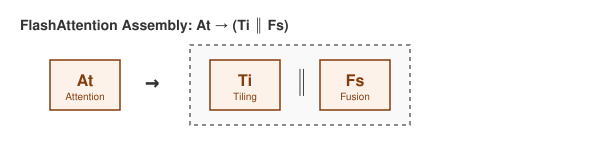
\includegraphics[width=0.85\columnwidth]{figures/system_assembly.pdf}}
    \caption{\textbf{FlashAttention assembly.} The algorithmic Attention (\texttt{At}) primitive composition links to runtime Tiling (\texttt{Ti}) and Kernel Fusion (\texttt{Fs}), keeping intermediates in SRAM rather than HBM.}
    \label{fig:flashattn}
\end{figure}

The remaining four walkthroughs test the framework on other constraint types (fragmentation, multi-device capacity), other hardware contexts (NVLink vs.\ InfiniBand, datacenter vs.\ edge), and its ability to rule candidates out as well as in. ZeRO-3 (\Cref{sec:zero-3}) tests a multi-device capacity constraint and demonstrates a cascade in which resolving one constraint introduces another. PagedAttention (\Cref{sec:paged-attention}) tests a fragmentation constraint, where simpler candidates such as Caching and Tiling fail their preconditions. Megatron-LM tensor parallelism (\Cref{sec:tensor-parallel}) tests the same constraint type as ZeRO-3 but with a different hardware context, and shows the framework selecting a different rewrite, the strongest evidence that the search is sensitive to hardware context, not just constraint type. The million-token edge case (\Cref{sec:edge-analysis}) tests the framework on an open deployment problem with three simultaneous binding constraints, and includes a dead-end analysis showing two plausible-but-wrong candidates pruned before a viable cascade emerges. Together the five derivation walkthroughs cover four constraint types and three hardware contexts, and they exercise both successful rewrites and pruned candidate rewrites. The Mamba case after them tests the grammar's boundary: a situation where the right answer changes the algorithm rather than refactoring the existing layout.

\subsection{ZeRO-3 Distributed Training}
\label{sec:zero-3}

ZeRO-3 \citep{rajbhandari2020} exercises the framework on a multi-device capacity constraint and demonstrates a \emph{constraint cascade}: resolving the initial capacity violation introduces a new bandwidth constraint, which the framework handles by composing two rewrites rather than one. The hardware context is a cross-node InfiniBand cluster, the opposite of the NVLink case we revisit in \Cref{sec:tensor-parallel}.

\subsubsection{Stage 1: The Na\"ive Assembly}

Na\"ive data-parallel training replicates the full model state on every device:
\begin{equation*}
M_{\text{naive-dp}} = [Pm \otimes Os \otimes Ad]_{\langle \cdot \rangle_{\text{Dr}}}^{\text{per device}} \rightarrow Vu \rightarrow Sy
\end{equation*}

\subsubsection{Stage 2: The Binding Constraint}

\begin{napkinmath}{ZeRO-3 memory budget}
For a 70B parameter model in mixed-precision training (Rule~1):
\begin{align*}
\text{mem}(Pm) &= 70\text{B} \times 2\;\text{bytes (FP16)} = \cvalint{\LLaMAWeightsGB}\;\text{GB} \\
\text{mem}(Ad) &= 70\text{B} \times 2\;\text{bytes (FP16)} = \cvalint{\LLaMAWeightsGB}\;\text{GB} \\
\text{mem}(Os) &= 70\text{B} \times 12\;\text{bytes}^{\dagger} = 840\;\text{GB}
\end{align*}

\footnotesize{${}^{\dagger}$Adam: FP32 copy (4B) + first moment (4B) + second moment (4B) = 12 bytes/param.}

\normalsize
\textbf{Total per-device:} $\cvalint{\LLaMAWeightsGB} + \cvalint{\LLaMAWeightsGB} + 840 = \cvalint{\ZeROMemGB}$\,GB.

\textbf{H100 HBM:} \cvalint{\HhHBMGB}\,GB. Exceeded by $\cvalint{\ZeROMinDevices}\times$.
\end{napkinmath}

\subsubsection{Stage 3: Rewrite Search}

\paragraph{Filter 1 (Layer).} HBM capacity, Hardware layer. Runtime candidates: $\{$Ti, Fs, Pf, Cc, Sc, Vr$\}$. Optimization-layer: $\{$Qz, Fc, Sy$\}$.

\paragraph{Filter 2 (Role).} Capacity $\Rightarrow$ Represent or Communicate. $\{$Ti, Vr, Cc, Qz, Fc, Sy$\}$.

\paragraph{Filter 3 (Constraint type).} Capacity exceeded, multi-device context: $\{$Sy, Vr, Qz, Fc$\}$.

\paragraph{Filter 4 (Hardware context).} Exact FP16 gradients required $\Rightarrow$ eliminate Qz. No general low-rank structure $\Rightarrow$ eliminate Fc. Vr addresses fragmentation, not aggregate capacity $\Rightarrow$ eliminate Vr.

\paragraph{Result.} \fbox{\texttt{Sync/Collective (Sy)}} (sharding), with \texttt{Prefetching (Pf)} as companion. This is the ZeRO rewrite \citep{rajbhandari2020}.

\subsubsection{Stage 4: The Optimized Assembly}

\begin{equation*}
M_{\text{ZeRO-3}} = \left[\underbrace{Pf \xrightarrow{bw} Sy}_{\text{gather } \ell{+}1} \;\parallel\; \underbrace{Vu}_{\text{compute } \ell}\right]^{L}
\end{equation*}
with residency $\langle Pm/N \otimes Os/N \otimes Ad/N \rangle_{\text{Dr}}$.

\begin{napkinmath}{ZeRO-3 compute vs.\ communication}
With $N = 16$ GPUs and a 70B model ($L = 80$ layers, ${\sim}$0.875B params/layer):

\textbf{All-gather time per layer (NVLink, 8 GPUs/node).} Ring all-gather transfers $\frac{N-1}{N}$ of the full tensor per device:
\begin{align*}
T_{\text{gather}}^{\text{NVL}}
&= \frac{7}{8} \cdot
   \frac{0.875\text{B} \times 2\;\text{bytes}}
        {\cvalint{\NVLinkBWGBs}\;\text{GB/s}} \\
&= \frac{7}{8} \cdot \frac{1.75\;\text{GB}}{900\;\text{GB/s}}
 \approx 1.7\;\text{ms}.
\end{align*}

\textbf{All-gather time per layer (InfiniBand, cross-node):}
\[
T_{\text{gather}}^{\text{IB}} = \frac{7}{8} \cdot \frac{1.75\;\text{GB}}{\cvalint{\IBBWGBs}\;\text{GB/s}} \approx 31\;\text{ms}
\]

\textbf{Compute time per layer} (forward + backward, batch size 4, seq len 4096):
\[
T_{\text{compute}} = \frac{6 \times 0.875 \times 10^9 \times 4 \times 4096}{\cvalint{\HhPeakTFLOPS} \times 10^{12}} \approx 87\;\text{ms}
\]

\textbf{Verdict:} NVLink: $T_{\text{compute}} \gg T_{\text{gather}}^{\text{NVL}}$, so prefetching fully hides communication. InfiniBand: margin is thin ($\sim$$2.8\times$). At smaller models, InfiniBand becomes the bottleneck, which is why ZeRO-3 uses gradient accumulation to increase $T_{\text{compute}}$.
\end{napkinmath}

Per-device memory drops to $\cvalint{\ZeROMemGB} / 16 = 70$\,GB, fitting comfortably in the \cvalint{\HhHBMGB}\,GB H100 HBM. But the optimized assembly reveals something the FlashAttention walkthrough did not: a \emph{constraint cascade}. Sharding the model state ($Sy$) resolved the capacity constraint ($\mid_{\text{cap}}$) but introduced a new bandwidth constraint ($\mid_{\text{bw}}$), every layer now needs to all-gather its weights from peer devices before it can compute. The framework's response was to compose two rewrites rather than one: $Sy$ for the capacity violation, $Pf$ (prefetching) to hide the new communication latency behind the previous layer's compute. The constraint operator generalizes naturally: $M \mid_{\text{cap}} \to M' \mid_{\text{bw}} \to M''$, with each violation triggering its own filter pass. This cascade pattern recurs in every multi-device walkthrough.

\subsection{PagedAttention}
\label{sec:paged-attention}

ZeRO-3 demonstrated the framework on a capacity constraint. PagedAttention demonstrates it on something the earlier examples do not exercise: a fragmentation constraint. Fragmentation is qualitatively different from capacity. The aggregate memory used is small, but the layout makes that memory unusable, the system has space but cannot allocate it contiguously. This forces the framework to select rewrites from a different region of the constraint-rewrite matrix (\Cref{tab:resolution-matrix}), and the four filters must distinguish between superficially similar candidates (Caching, Tiling, Virtualization) that have very different preconditions.

\subsubsection{Stage 1: The Na\"ive Assembly}

During autoregressive generation, each request maintains a contiguous KV-cache in HBM:
\begin{equation*}
M_{\text{naive-serve}} = Hs_{\langle \text{Dr},\, \text{contig} \rangle} \rightarrow At \rightarrow Dd \;\bigm|_{\text{alloc}}
\end{equation*}
with the allocation constraint $\text{alloc} = \text{contiguous}$.

\subsubsection{Stage 2: The Binding Constraint}

For a 70B dense-MHA model with 80 layers and 64 attention heads of dimension 128 (dense multi-head attention, not the grouped-query variant in Llama-70B), each token's KV-cache entry consumes $2 \times 80 \times 64 \times 128 \times 2 = 2.5$\,MB. A request with maximum context 8,192 tokens requires $\sim$20\,GB of contiguous HBM, but may only generate 500 tokens. Fragmentation:
\begin{equation*}
\text{Fg} = \frac{\text{allocated} - \text{used}}{\text{allocated}} = \frac{20 - 1.25}{20} \approx 94\%
\end{equation*}

With 4 concurrent requests, 80\,GB is allocated, exhausting the H100's \cvalint{\HhHBMGB}\,GB HBM, though only $\sim$5\,GB is used.

\subsubsection{Stage 3: Rewrite Search}

\paragraph{Filters 1--3.} Fragmentation constraint $\Rightarrow$ Runtime layer, Represent/Control roles: $\{$Vr, Cc, Sc$\}$.

\paragraph{Filter 4 (Hardware context).} Preconditions against $\mathcal{P} = \{$variable-length, dynamically-growing, request-isolated$\}$:
\begin{itemize}[nosep]
\item \textbf{Caching (Cc):} preconditions $= \{$temporal-reuse$\}$. KV entries are written once per token and read once during attention; there is no reuse pattern Cc could exploit. Eliminated.
\item \textbf{Scheduler (Sc):} preconditions $= \{$batch-formable workloads$\}$. Sc resolves utilization, not allocation; the fragmentation persists regardless of scheduling order. Eliminated.
\item \textbf{Virtualization (Vr):} preconditions $= \{$variable-length-data, dynamically-growing$\}$. The KV-cache satisfies both. Retained.
\end{itemize}

\paragraph{Result.} \fbox{\texttt{Virtualization (Vr)}}. The filters select virtualization to map logical blocks to non-contiguous physical pages. This is the PagedAttention rewrite \citep{kwon2023}.

\subsubsection{Stage 4: The Optimized Assembly}

\begin{equation*}
M_{\text{paged}} = Hs \rightarrow Vr \rightarrow Cc_{\langle \text{pages} \rangle_{\text{Dr}}} \rightarrow Sc
\end{equation*}

Fragmentation drops from $>90\%$ to $<4\%$ \citep{kwon2023}. Virtualization decouples logical structure from physical layout, the same principle that motivated virtual memory in operating systems half a century ago, now applied to GPU HBM half a century later. The structural similarity is not coincidence: both arise when a fixed physical resource must serve dynamically-sized, dynamically-arriving requests. The framework surfaces this connection naturally because Vr's metadata (preconditions $=$ \{variable-length-data, dynamically-growing\}) encodes the abstract pattern, not the implementation.

\subsection{Tensor Parallelism}
\label{sec:tensor-parallel}

The third walkthrough is the most pointed test of the framework's claim to be sensitive to hardware context. The constraint type is identical to ZeRO-3's: multi-device capacity, but the deployment context is different: a small, NVLink-connected cluster doing inference rather than a large, InfiniBand-connected one doing training. Identical constraint, different hardware: should the framework propose a different rewrite? It should, and it does. This walkthrough shows the four filters surfacing tensor parallelism (Megatron-LM) instead of ZeRO sharding, with the divergence happening entirely at Filter 4 (hardware context). If the framework were merely a constraint-to-technique lookup table, this discrimination would be impossible.

\subsubsection{Stage 1: The Na\"ive Assembly}

Inference of a 70B model on a single device:
\begin{equation*}
M_{\text{naive-infer}} = Pm_{\langle \text{Dr} \rangle} \rightarrow [Dd \rightarrow \mathrm{softmax} \rightarrow Dd]^{L}
\end{equation*}

\subsubsection{Stage 2: The Binding Constraint}

\begin{napkinmath}{Tensor parallelism capacity constraint}
\textbf{Model weights:} 70B $\times$ 2 bytes (FP16) = \cvalint{\LLaMAWeightsGB}\,GB.

\textbf{Single H100 HBM:} \cvalint{\HhHBMGB}\,GB.

\textbf{Deficit:} $\cvalint{\LLaMAWeightsGB} / \cvalint{\HhHBMGB} = 1.75\times$ oversubscription. The model does not fit on one device, even before KV-cache and activation memory.

The constraint is \textbf{capacity (multi-device)}: weights must be distributed across devices.
\end{napkinmath}

\subsubsection{Stage 3: Rewrite Search}

\paragraph{Filter 1 (Layer).} HBM capacity, Hardware layer. Runtime + Optimization candidates.

\paragraph{Filter 2 (Role).} Capacity $\Rightarrow$ Represent or Communicate: $\{$Sy, Vr, Qz, Fc, Ti$\}$.

\paragraph{Filter 3 (Constraint type).} Capacity exceeded, multi-device: $\{$Sy, Vr, Qz$\}$.

\paragraph{Filter 4 (Hardware context).} Inference requires exact weights (no training tolerance for quantization noise at this scale) $\Rightarrow$ Qz is a secondary option. KV-cache is not the bottleneck here $\Rightarrow$ Vr does not address weight capacity. NVLink cluster with $N = \cvalint{\TPdevices}$ GPUs available.

\paragraph{Result.} \fbox{\texttt{Sync/Collective (Sy)}}. Specifically, column-parallel weight sharding with all-reduce after each layer's forward pass. This is Megatron-LM tensor parallelism \citep{shoeybi2019megatron}.

\subsubsection{Stage 4: The Optimized Assembly}

\begin{equation*}
M_{\text{TP}} = [(Pm/N)_{\langle \text{Dr} \rangle} \rightarrow Dd \rightarrow Sy_{\text{all-reduce}}]^{L}
\end{equation*}

\begin{napkinmath}{Tensor parallelism communication overhead}
With $N = \cvalint{\TPdevices}$ GPUs on NVLink (\cvalint{\NVLinkBWGBs}\,GB/s):

\textbf{Per-device weights:} $\cvalint{\LLaMAWeightsGB} / \cvalint{\TPdevices} = \cval{\TPweightsPerDevice}$\,GB. Fits in \cvalint{\HhHBMGB}\,GB HBM.

\textbf{Per-layer weights to stream from HBM:} $\cval{\TPweightsPerDevice}$\,GB / 80 layers $\approx 219$\,MB per layer per device.

\textbf{HBM-bound time per layer (decode, $B{=}1$):} At decode time the matmul is bandwidth-bound, not compute-bound: every layer must read its shard of weights from HBM at \cval{\HhBWTBs}\,TB/s.
\begin{align*}
T_{\text{HBM}} &= \frac{219\;\text{MB}}{\cval{\HhBWTBs}\;\text{TB/s}} \approx 65\;\mu\text{s per layer}
\end{align*}

\textbf{All-reduce per layer.} Each transformer layer produces a hidden-state output of dimension $h = 8192$. The all-reduce volume is $|Y| = B \cdot s \cdot h \cdot 2$\,bytes; for $B = s = 1$ this is 16\,KB. Ring all-reduce ($\gamma = 2(N{-}1)/N = 1.75$):
\begin{align*}
T_{\text{AR}}^{\text{NVL}} &= \gamma \cdot \tfrac{16\;\text{KB}}{\cvalint{\NVLinkBWGBs}\;\text{GB/s}} + 1\;\mu\text{s} \approx 1.03\;\mu\text{s}
\end{align*}

\textbf{Ratio:} $T_{\text{HBM}} / T_{\text{AR}}^{\text{NVL}} \approx 63\times$. NVLink communication is roughly 1.5\% of layer time at decode. Negligible.

\textbf{On InfiniBand} (50\,GB/s, ${\sim}9$\,$\mu$s end-to-end including software stack): $T_{\text{AR}}^{\text{IB}} \approx 10\;\mu$s. The ratio drops to $\sim$6.5$\times$, communication becomes a measurable 15\% overhead, and the case for keeping TP inside the NVLink domain becomes clear.
\end{napkinmath}

The framework derives not only the rewrite (sharding) but also the topology constraint (NVLink-connected devices) from the bandwidth analysis itself. Tensor parallelism across InfiniBand is possible but inefficient; the napkin math reveals why practitioners keep TP within an NVLink domain and use pipeline or data parallelism across nodes \citep{narayanan2021}.

\subsection{Million-Token Context on Edge}
\label{sec:edge-analysis}

We apply the framework to serving a model with \EdgeCtxTokens{}-token context on a unified-memory edge device (Apple M4 Pro: \cvalint{\EdgeRAMGB}\,GB unified RAM, \cvalint{\EdgeBWGBs}\,GB/s bandwidth, an approximate \cvalint{\EdgeTFLOPS}\,TOPS of aggregate compute across GPU and Neural Engine).

\begin{napkinmath}{Million-token KV-cache on edge}
For a 7B model (32 layers, 32 KV-heads, head dim 128):

\textbf{KV per token:} $2 \times 32 \times 32 \times 128 \times 2 = \cval{\EdgeKVPerTokenMB}$\,MB.

\textbf{KV at \EdgeCtxTokens{} tokens:}
\[
\cval{\EdgeKVPerTokenMB}\;\text{MB} \times \EdgeCtxTokensRaw{} = \EdgeKVTotalGB{}\;\text{GB}
\]

\textbf{Exceeds \cvalint{\EdgeRAMGB}\,GB unified memory by ${\sim}13\times$.}

Three constraints bind simultaneously:
\begin{enumerate}[nosep]
\item \textbf{Capacity:} KV-cache exceeds memory by $13\times$.
\item \textbf{Bandwidth:} \cvalint{\EdgeBWGBs}\,GB/s is $12\times$ slower than H100 HBM; streaming full KV per token takes ${\sim}1.7$\,s.
\item \textbf{Compute:} $O(n^2)$ attention at this scale on \cvalint{\EdgeTFLOPS}\,TOPS is catastrophic.
\end{enumerate}
\end{napkinmath}

\paragraph{Constraint-driven search.} We show the search tree with its dead ends, the part of the derivation that prunes wrong paths with napkin math before an engineer would waste time implementing them.

\begin{errorcase}{Dead end 1: Ring Attention on M4 Pro}
\textbf{Candidate.} The heuristic's capacity filter surfaces Ring Attention \citep{liu2023ring} as a rewrite for the $O(n^2)$ memory constraint: distribute the KV-cache across devices via a ring of attention tiles.

\textbf{Why it fails.} Ring Attention requires multiple devices with high-bandwidth interconnect. The M4 Pro is a single SoC. There is no ring. Even if we treated CPU and GPU as separate ``devices,'' the M4 Pro's unified memory architecture means there is no bandwidth gain from partitioning, both access the same \cvalint{\EdgeBWGBs}\,GB/s memory bus.

\textbf{Filter 4 (Hardware context):} $\text{RingAt}.\text{preconditions} = \{$multi-device, point-to-point interconnect$\}$. $\{$multi-device$\} \not\subseteq \mathcal{P}_{\text{M4 Pro}}$. Eliminated.

\textbf{Napkin math confirms:} Even hypothetically, ring communication across Thunderbolt ($\sim$5\,GB/s) would add roughly $\EdgeKVTotalGB{}\,\text{GB} / 5\,\text{GB/s} \approx 98$\,s per token. Catastrophic. Pruned.
\end{errorcase}

\begin{errorcase}{Dead end 2: Tiling alone (FlashAttention-style)}
\textbf{Candidate.} Tiling resolved the attention memory bottleneck on H100 (\Cref{sec:walkthrough}). Can it work here?

\textbf{Why it is insufficient.} Tiling reduces intermediate memory ($S = QK^T$) from $O(n^2)$ to $O(B^2)$. But the KV-cache itself ($\EdgeKVTotalGB$\,GB) is not an intermediate; it is state that must persist across tokens. Tiling does not reduce persistent state.

\textbf{Napkin math:} After tiling, intermediate memory drops to $\sim$128\,KB per tile. But KV-cache remains at $\EdgeKVTotalGB$\,GB. The capacity constraint is still violated by $13\times$. Tiling is necessary but not sufficient, it must be combined with KV compression.
\end{errorcase}

\paragraph{The viable cascade.} After pruning Ring Attention and standalone Tiling, the heuristic produces a cascade of rewrites, each resolving one constraint while possibly introducing another:

\begin{itemize}[nosep]
\item \textbf{Capacity (first pass):} Qz (quantize KV to INT4: $4\times$ reduction $\Rightarrow$ 122\,GB). Still exceeds \cvalint{\EdgeRAMGB}\,GB.
\item \textbf{Capacity (second pass):} Fc (low-rank KV approximation: $2\times$ $\Rightarrow$ 61\,GB). Still $1.7\times$ over.
\item \textbf{Capacity (third pass):} Vr (disk-backed paging: active working set $\sim$4\,GB fits in RAM).
\item \textbf{Bandwidth:} Pf (prefetch next context window from SSD during compute).
\item \textbf{Compute:} The $O(n^2)$ cost at this scale requires a sub-quadratic attention mechanism, an Algorithm-layer substitution. Candidates: sparse attention ($O(n \sqrt{n})$), linear attention ($O(n)$).
\end{itemize}

\paragraph{The final assembly.}

\begin{equation*}
M_{\text{edge}} = [Ti \rightarrow (Dd_{\text{sparse}} \rightarrow \mathrm{softmax})_{\langle\text{Sr}\rangle}]^{n/B} \rightarrow Fs
\end{equation*}
with KV residency:
\begin{equation*}
Hs \rightarrow Qz_{\text{INT4}} \rightarrow Fc \rightarrow Vr_{\langle\text{SSD} \to \text{RAM}\rangle} \rightarrow Pf
\end{equation*}

\begin{napkinmath}{Closed-loop edge verification}
\textbf{After INT4 quantization + $2\times$ factorization:}
\[
\text{KV}_{\text{compressed}} = \frac{\EdgeKVTotalGB{}}{4 \times 2} = 61\;\text{GB}
\]

Still $1.7\times$ over \cvalint{\EdgeRAMGB}\,GB. Virtualization (Vr) pages the overflow to SSD; active working set per decode step: ${\sim}$4\,GB (recent context window).

\textbf{Bandwidth after compression:} Streaming 4\,GB working set:
\[
T_{\text{stream}} = \frac{4\;\text{GB}}{\cvalint{\EdgeBWGBs}\;\text{GB/s}} \approx 15\;\text{ms/token}
\]

\textbf{With sub-quadratic attention} ($O(n\sqrt{n})$ compute, $\sqrt{10^6} = 1000$ effective attention reach per decode step): once attention cost is sub-quadratic, decode compute per token is dominated by the linear layers at $2P$:
\[
T_{\text{compute}} \approx \frac{2 \times 7 \times 10^9}{\cvalint{\EdgeTFLOPS} \times 10^{12}} \approx 0.26\;\text{ms per token}
\]
(Attention contributes roughly $2\, w\, d\, \text{heads}\, \text{layers} \approx 0.26$\,GFLOP per token on this 7B configuration, about $2\%$ of the 14\,GFLOP linear budget, so we drop it.)

\textbf{Bottleneck:} Memory bandwidth at 15\,ms/token ($\sim$67 tokens/s). Acceptable for edge serving, and the binding constraint is now bandwidth rather than the original capacity-and-compute pile-up.

\textbf{Structural prediction:} Any viable million-token edge solution will contain \{Qz, Fc, Vr, Pf, sub-quadratic At\} or their functional equivalents. A paper that achieves this without one of these components must have found a qualitatively different approach.

\textbf{What the dead ends prove:} The framework did not merely list the answer, it pruned Ring Attention (wrong hardware context) and standalone Tiling (wrong constraint scope) before arriving at the viable cascade. Showing the search tree's pruned branches is what distinguishes a generative framework from a retrospective labeling scheme.
\end{napkinmath}

On the unsolved edge problem, the framework produced a structurally specified assembly, predicted the components any viable solution must contain, and showed the wrong paths it considered before arriving at the cascade. ``Generative'' here does not mean the framework outputs the answer; it means the framework narrows the answer space tightly enough that any viable answer must contain (or functionally substitute for) the structural ingredients we predicted.

\subsection{An Honest Failure: Mamba}
\label{sec:mamba-failure}

The preceding five walkthroughs all succeed. That could mean the framework is genuinely generative, or it could mean we selected cases the framework was designed to handle. The honest test is a boundary case where we know in advance the framework will fail, and we examine exactly where in the filter chain the failure surfaces. We use Mamba and other state-space models as that failure case.

\paragraph{Stage 1: the na\"ive assembly.} Decode-time attention on a long-context Transformer has the assembly $M_{\text{decode}} = \text{At}\rightarrow \text{FFN}$, with attention materializing an $O(n)$ KV state that must be streamed from HBM at every decode step. At long context, the KV stream dominates decode time.

\paragraph{Stage 2: the binding constraint.} For a 70B model at 128K context, per-token KV stream is $2\cdot 80\cdot 8\cdot 128\cdot 128{,}000\cdot 2 \approx 42$\,GB. Even when capacity is handled by sharding, each decode step must read the resident KV state. The binding constraint is $\text{HBM-bandwidth}$: attention is reading KV state at the ceiling of the memory system, and arithmetic intensity stays fixed below ridge regardless of tile size. $M_{\text{decode}} \mid_{\text{BW}}$.

\paragraph{Stage 3: the constraint-driven search.} We run the four filters against the HBM-bandwidth violation.

\begin{itemize}[nosep, leftmargin=*]
\item \textbf{Filter 1 (Layer).} Bandwidth violation at Hardware $\Rightarrow$ Runtime and Optimization candidates: $\{$Ti, Fs, Pf, Cc, Sc, Vr, Qz, Fc$\}$.
\item \textbf{Filter 2 (Role).} Bandwidth pressure favors Represent (reduce bytes moved) or Compute (fuse work into fewer reads): $\{$Ti, Fs, Vr, Cc, Qz, Fc$\}$.
\item \textbf{Filter 3 (Constraint type).} Bandwidth at the HBM ceiling, not capacity, not fragmentation: $\{$Fs, Qz, Fc$\}$. Tiling does not reduce total bytes moved during decode; Virtualization addresses fragmentation, not aggregate bandwidth.
\item \textbf{Filter 4 (Hardware context).} Decode must read the full KV-cache once per token regardless of how the computation is scheduled or how precisely weights are stored. Fusion, Quantization, and Factorization all reduce \emph{weight} or \emph{activation} memory traffic; none of them changes the KV-cache traffic that dominates decode at 128K context.
\end{itemize}

\paragraph{What the filters return.} The best the search produces is a cascade (Qz + Fs + Pf) that reduces \emph{weight} streaming and overlaps it with compute, but leaves the KV-cache stream untouched. Decode time drops by a modest factor tied to weight-byte savings and stalls again at the KV bandwidth ceiling as context length grows. The filter chain cannot return an assembly that removes the KV stream, because no rewrite rule in $R$ is allowed to replace the attention interaction with a different algorithmic mechanism that trades $O(n)$ KV state for an $O(1)$ recurrent state.

\paragraph{Why the framework fails here.} Mamba, and state-space models more broadly \citep{gu2023mamba}, resolve the constraint by changing the algorithmic assembly rather than by refactoring the existing attention layout. The long-context interaction is no longer expressed as Attention ($\text{At}$) over a growing KV state; it is expressed as a recurrent state-space assembly with bounded State ($\text{St}$). In our notation:
\begin{equation*}
M_{\text{mamba}} = \text{St} \rightarrow \text{FFN},
\end{equation*}
with $\text{St}$ carrying bounded memory regardless of sequence length. The Constraint-Driven Rewrite Search cannot generate this assembly because the search operates on rule metadata for rewrites that preserve the primitives in the naive assembly. Replacing the attention interaction with recurrent state-space dynamics changes what the assembly computes, not where it stores intermediates or how it schedules them. The grammar can admit the new primitive relation through the Irreducibility Criterion, but the four filters cannot propose it as a bandwidth-preserving layout rewrite. Speculative decoding (trading verification compute for serial latency) and Mixture-of-Experts routing (trading dense compute for conditional compute) fail for the same reason and are summarized in \Cref{fig:mamba}.

\paragraph{What the failure proves about scope.} The scope of the framework is now precise. The Constraint-Driven Rewrite Search derives architectural rewrites that preserve the semantic primitives in the na\"ive assembly and refactor their data layout, scheduling, precision, or memory residency. It does not derive rewrites that replace one algorithmic interaction with another; those are algorithmic innovations by definition, and adopting one requires updating the primitive vocabulary or the admissible assembly patterns. When a new algorithmic assembly is proposed (Mamba's recurrent state-space block, Hyena's long convolution, a Mixture-of-Experts router), the framework absorbs it either by composing existing primitives differently or by admitting a new primitive through the Irreducibility Criterion (\Cref{sec:irreducibility}), after which the filter search can compose assemblies that use it. The framework is generative over layout refactorings, not over algorithm design.

Across the five successful derivations and the Mamba boundary test, the same four-filter procedure operated on the same primitive vocabulary and rewrite rule set and produced five viable assemblies plus one honest failure. The differences trace cleanly to the inputs: different constraint type (capacity vs.\ fragmentation vs.\ bandwidth), different scope (single-device vs.\ multi-device), different hardware context (NVLink vs.\ InfiniBand vs.\ unified memory), different interaction shape (single rewrite vs.\ cascade vs.\ simultaneous constraints). In every case the filter steps were deterministic, the eliminations were justified by metadata, and the output, viable or infeasible, came from operating on the grammar rather than recalling a known answer. The framework does not need to know about FlashAttention to produce its rewrite; it needs to know about Tiling, Fusion, SRAM, and the irreducibility of Attention.

% ============================================================================
\section{Probabilistic Constraints}
\label{sec:probabilistic}

Every walkthrough so far has assumed a determinism that the fleet breaks: a single node, a single constraint, a single bound that is either satisfied or violated. That assumption is what made the four-filter search tractable. It also fixes the scope. Once the job spans hundreds of nodes, no bound is deterministic anymore: each constraint fires with some probability on each step, and the question is no longer whether the constraint holds but how often it fails. A system that works on 8 GPUs and fails at 1{,}024 has not encountered an unusual condition; it has encountered the normal operating regime of distributed training. This section extends the constraint operator to that regime.

\subsection{The Generalized Constraint Operator}

In \Cref{sec:composition}, we introduced the generalized constraint operator:
\begin{equation}
M \;\mid_{C,\; p > \theta} \quad \xRightarrow{\;P(C\text{ violated}) > \theta\;} \quad \text{\textsc{Search}}(M, C) = M'
\end{equation}
For deterministic constraints ($\theta = 0$), any violation triggers search; this is the regime of \Cref{sec:walkthrough}. For probabilistic constraints ($\theta > 0$), the trigger is a probability threshold. The relevant measurements are no longer just mean latency or nominal bandwidth; \texttt{Latency (La)} and \texttt{Availability (Av)} must be interpreted as tail distributions that determine $P(C\text{ violated})$.

\subsection{The Straggler Problem}

\begin{errorcase}{Stragglers in distributed all-reduce}
\textbf{Scenario.} A 1,024-GPU training job runs ring all-reduce across 128 nodes. The deterministic model (Rule~4) predicts:
\begin{align*}
T_{\text{all-reduce}} &= \gamma \cdot \frac{|G|}{bw} + \alpha \\
&= \tfrac{2 \times 1023}{1024} \cdot \tfrac{26\;\text{GB}}{50\;\text{GB/s}} + 5\;\mu\text{s} \\
&\approx 1.04\;\text{s}
\end{align*}

\textbf{What actually happens.} At 1,024 GPUs, the probability that at least one node experiences a transient slowdown per step:
\begin{align*}
P(\text{straggler}) &= 1 - (1 - p)^{128} \\
&\approx 1 - (0.99)^{128} \approx 72\%
\end{align*}

A single straggler running $3\times$ slower turns $T_{\text{all-reduce}}$ from 1.04\,s to 3.1\,s. The deterministic framework misses this because $\mid_C$ assumes deterministic bounds. Straggler effects are probabilistic: $P(\text{violation}) > 0$ even when $\text{mean}(C)$ is satisfied.
\end{errorcase}

\subsection{Applying the Generalized Operator}

Setting $\theta = 0.5$: when $P(\text{straggler}) = 72\% > \theta$, the generalized constraint operator fires. The four-filter heuristics correctly surface Control-role rewrites:

\begin{napkinmath}{Straggler mitigation cost}
\textbf{Without mitigation:} Expected per-step time:
\[
E[T] = 0.28 \times 1.04 + 0.72 \times 3.1 \approx 2.5\;\text{s}
\]

\textbf{With redundant computation (2\% overhead):} Launch backup all-reduce on alternate paths; the faster path completes. Expected time drops to about 1.1\,s, a $2.3\times$ improvement for 2\% compute overhead.

\textbf{Filter result:} Layer $\to$ Production/Runtime. Role $\to$ Control. Hardware context $\to$ multi-node with synchronization barrier. Candidates: \textbf{Sc} (topology-aware scheduling), \textbf{Oc} (redundant execution, bounded staleness). This matches Google's production approach \citep{dean2013}.
\end{napkinmath}

\paragraph{The boundary.} The deterministic framework (\Cref{sec:walkthrough}) is accurate within one node and progressively less so as fleet size grows. The generalized operator formalizes where the boundary lies ($P(\text{straggler}) > \theta$) and what replaces the deterministic trigger. Fully integrating probabilistic constraints into the cost rules, so that tail-latency and straggler distributions participate in the four-filter search as first-class inputs, is the most important open formalization challenge.

% ============================================================================
\section{Teaching with the Framework}
\label{sec:teaching}

The previous sections built the framework as a research artifact: a design space, a search heuristic, and a cost calculus. This section reframes the same machinery as a curriculum. The things built for derivation (irreducibility, four filters, cost rules) turn out to be exactly the things students need to develop transferable intuition.

The section unfolds in three movements. First, we distill the framework into manipulable equations and a structured whiteboard protocol that students can apply by hand (\Cref{sec:iron-laws,sec:whiteboard}). Second, we work through examples that show what teaching with these tools looks like in practice: a routine sizing problem, a forward-derivation exercise, and a failure case where the filters catch a wrong answer (\Cref{sec:kv-sizing,sec:predict-paper,sec:failure-case}). Third, we present the curricular machinery: an exercise bank graded from single-node to fleet-scale, integration with two existing platforms, and preliminary deployment evidence from a Harvard course (\Cref{sec:exercises,sec:curriculum,sec:deployment}). The thread connecting all three is that every step of the framework (a constraint, a filter, a primitive) is an item a student can name, manipulate, and defend at a whiteboard. The pedagogy is not added on top; it is the same machinery rotated toward learning.

\subsection{Three First-Order Bounds}
\label{sec:iron-laws}

Patterson and Hennessy's Iron Law of processor performance \citep{hennessy2019architecture}, $\text{Time} = \text{IC} \times \text{CPI} \times T_{\text{clk}}$, is the canonical example of a manipulable equation: it decomposes execution time into three independent terms a student can substitute, hold constant, and reason about. We do not claim the same algebraic identity for ML systems performance, but we do offer three back-of-envelope bounds in the same spirit. They are not identities; they are inequalities. They do not decompose a single observable quantity into independent terms; they describe which constraint binds first as parameters scale. Students can still substitute hardware specifications and solve for the binding constraint, which is what the manipulable form is for.

\paragraph{Bound 1: Memory Capacity.} A workload fits on $N$ devices if and only if:
\begin{align}
\label{eq:iron-capacity}
&\underbrace{P \cdot b_w}_{\text{weights}} \;+\; \underbrace{P \cdot b_o}_{\text{optimizer}} \;+\; \underbrace{B \cdot s \cdot h \cdot L \cdot b_a}_{\text{activations}} \notag \\
&\quad +\; \underbrace{2 \cdot L \cdot n_{\text{kv}} \cdot d \cdot s \cdot b_k}_{\text{KV-cache}} \;\leq\; N \cdot C_{\text{HBM}}
\end{align}
where $P$ is parameters, $b_w$ is bytes per weight, $b_o$ is bytes per optimizer state (12 for Adam), $B$ is batch size, $s$ is sequence length, $h$ is hidden dimension, $L$ is layers, $n_{\text{kv}}$ is KV-heads, $d$ is head dimension, $b_a$ and $b_k$ are bytes per activation and KV entry, and $C_{\text{HBM}}$ is per-device HBM capacity. Each term maps to a Represent-role primitive; each $\leq$ is a constraint operator $\mid_{\text{CAP}}$. Not every term coexists in practice. The optimizer term ($P \cdot b_o$) and activation term apply only during training; the KV-cache term applies only during autoregressive inference. Bound 1 is a pedagogical superset that a student specializes to a specific workload by dropping the inapplicable terms.

\paragraph{Bound 2: Throughput.} Per-token throughput is:
\begin{equation}
\label{eq:iron-throughput}
\text{Tokens/s} \;=\; \bigl[\, T_{\max} + \delta_{\text{bubble}} \,\bigr]^{-1},
\end{equation}
where $T_{\max}$ is the binding-constraint time:
\begin{equation}
\label{eq:iron-throughput-tmax}
T_{\max} = \max\!\left(\underbrace{\tfrac{2P}{N \pi}}_{\text{compute}},\;\; \underbrace{\tfrac{P \cdot b_w}{N \beta}}_{\text{bandwidth}},\;\; \underbrace{\tfrac{\gamma |G|}{bw_{\text{net}}}}_{\text{comm}}\right).
\end{equation}
where $\pi$ is per-device peak FLOP/s, $\beta$ is memory bandwidth, $bw_{\text{net}}$ is network bandwidth, $|G|$ is gradient size, $\gamma$ is the collective scaling factor, and $\delta_{\text{bubble}}$ is the pipeline bubble overhead from \Cref{eq:bubble}. The $\max$ identifies the binding constraint; the additive $\delta_{\text{bubble}}$ captures the concurrency overhead that simpler models ignore. The compute term shown ($2P$) is the inference forward-pass form; training replaces it with $6P$ to account for backward-pass cost, and the gradient-communication term drops out entirely during inference.

\paragraph{Bound 3: Serving Efficiency.} For inference, the arithmetic intensity is:
\begin{equation}
\label{eq:iron-serving}
I = \frac{2P \cdot B}{P \cdot b_w} = \frac{2B}{b_w} \;\text{FLOP/byte}
\end{equation}
At batch size $B = 1$ with FP16 weights ($b_w = 2$): $I = 1$ FLOP/byte. The ridge point on H100 is 295. The system is $295\times$ below peak, and the only lever is $B$. This is why continuous batching exists: it is not a software optimization but a physical necessity for efficient hardware utilization.

\paragraph{Why three laws are enough.} Capacity, throughput, and serving efficiency are not arbitrary choices. Capacity is the constraint that fails first (the model must fit before anything else matters); throughput is the constraint that determines training cost (which is what funds the next model); and serving efficiency is the constraint that determines inference economics (which is what funds the next deployment). Every other ML systems equation a student is likely to encounter: scaling laws, FLOP-utilization estimates, latency budgets, is a special case of one of these three. Treating them as the first equations on the whiteboard means students learn a small, complete vocabulary that generalizes, rather than a sprawling collection of named formulas.

\subsection{The Whiteboard Protocol}
\label{sec:whiteboard}

These bounds give students the equations; the whiteboard protocol gives them the procedure. In classroom and interview settings, the four-stage walkthrough used throughout \Cref{sec:walkthrough} becomes a four-step protocol that an instructor can use to lead a discussion or that a candidate can use to structure an answer:

\begin{enumerate}[nosep, leftmargin=*]
\item \textbf{Write the na\"ive assembly.} Decompose the system into irreducible primitives.

\item \textbf{Annotate with hardware specs and compute costs.} Attach memory residency, apply Rules 1--4.

\item \textbf{Run the four filters.} Write the candidate set and cross out primitives as each filter prunes. This makes reasoning visible and debuggable.

\item \textbf{Verify the optimized assembly.} Re-evaluate Rules 1--4. Confirm the constraint is resolved. Check for cascading constraints.
\end{enumerate}

The protocol's power lies in Step~3: when a student crosses out ``Caching (Cc)'' because the access pattern has no temporal reuse, they are learning a transferable principle about memory hierarchies, not memorizing a FlashAttention-specific fact. The crossing-out is observable: an instructor can see exactly which filter each student misapplies, and the student can see exactly where their reasoning diverged from the correct chain. This is the diagnostic value the framework adds to existing instruction.


\subsection{Worked Example: KV-Cache Sizing}
\label{sec:kv-sizing}

\paragraph{Problem.} ``You are serving a 7B model (32 layers, 32 KV-heads, head dim 128) on a single GPU with 24\,GB VRAM. Weights consume 14\,GB in FP16. How many concurrent requests at context length 4,096 can you serve?''

\begin{napkinmath}{KV-cache sizing}
\textbf{Step 1: Na\"ive assembly.}
\[
M = [Hs_{\text{contig}} \otimes Pm]_{\langle \cdot \rangle_{\text{Dr}}} \rightarrow At^L
\]

\textbf{Step 2: Hardware annotation.}
\begin{align*}
\text{Available VRAM} &= 24 - 14 = 10\;\text{GB} \\
\text{KV per token} &= 2 \times 32 \times 32 \times 128 \times 2 = 0.5\;\text{MB} \\
\text{KV per request} &= 0.5 \times 4{,}096 = 2{,}048\;\text{MB} \approx 2\;\text{GB} \\
\text{Max concurrent} &= \lfloor 10 / 2 \rfloor = \mathbf{5}
\end{align*}

\textbf{Step 3: Fragmentation.} With contiguous allocation and variable-length requests (some use 512 of 4,096 tokens): $\text{Fg} \approx 87\%$. Effective concurrency: \textbf{1--2 requests}.

\textbf{Four filters:} Layer $\to$ Runtime. Role $\to$ Represent/Control. Constraint $\to$ Fragmentation. Hardware $\to$ single GPU, variable-length state.

\textbf{Result:} \textbf{Vr} + \textbf{Cc}. With paged allocation, fragmentation $<4\%$:
\[
\text{Concurrent requests} = \left\lfloor \frac{10{,}240\;\text{MB}}{0.5 \times 512} \right\rfloor = \mathbf{40}
\]

An $8\times$ improvement. \textbf{Cascade check:} 40 requests raises compute demand $\Rightarrow$ continuous batching needed.
\end{napkinmath}

The KV-cache exercise is routine in its arithmetic but instructive in its structure. A student who has never seen PagedAttention by name still arrives at it in five whiteboard steps, along with the cascade that follows. The exercise is also the first place where the student experiences the cascade pattern directly: resolving fragmentation immediately reveals a downstream compute constraint, exactly as the multi-device walkthroughs demonstrated. The lesson is structural: one fix is rarely the whole story.

\subsection{The ``Predict the Paper'' Exercise}
\label{sec:predict-paper}

The KV-cache example tested the framework as a sizing tool. The next exercise tests it as a derivation tool, which is the more demanding claim, because it asks students to produce a system that they have not yet seen and then verify their answer against the published literature. We call this exercise ``Predict the Paper,'' and it is the strongest pedagogical demonstration of the framework's generative claim. Given only a constraint, a hardware specification, and the four filters, students should be able to derive the architecture of a published system before the instructor reveals its name.

\paragraph{Setup.} ``Autoregressive decoding of a 70B model on a single H100: 12 tokens/s, of which 80\,ms is memory-bandwidth-bound (streaming 140\,GB weights at \cval{\HhBWTBs}\,TB/s). GPU compute is 96\% idle. Design a system achieving 100+ tokens/s.''

\begin{napkinmath}{Predict the paper: batched decoding}
\textbf{Root cause:} Arithmetic intensity at $B = 1$:
\[
I = \frac{2 \times 70 \times 10^9}{140 \times 10^9} = 1\;\text{FLOP/byte}
\]

Ridge point = 295. The kernel is $295\times$ below, massively memory-bound.

\textbf{Roofline insight:} Batching $B$ requests amortizes weight reads:
\[
I_{\text{batched}} = B \;\text{FLOP/byte}
\]

At $B = 295$, the workload reaches the ridge point.

\textbf{Filter result:} Utilization $\Rightarrow$ Sc (iteration-level scheduler). Companion: Vr (PagedAttention for managing concurrent KV-caches).
\end{napkinmath}

The instructor reveals: this is Orca/vLLM \citep{yu2022orca, kwon2023}. Students experience the critical insight: they derived a published system from constraints, without knowing its name in advance. The point is not that the framework is sufficient to invent these systems. Real research involves trial, error, and engineering judgment we have not formalized, but that the framework narrows the design space tightly enough that students arrive at the same general class of solution as the published authors. The rewrite is no longer mysterious; it is mechanically motivated.

A natural question follows: what happens when students propose the wrong rewrite? The framework's value depends on whether it catches mistakes as crisply as it derives correct answers. The next subsection shows exactly that.

\subsection{Failure Case}
\label{sec:failure-case}

\begin{errorcase}{Student applies wrong rewrite to attention bottleneck}
\textbf{Scenario.} A student proposes \textbf{Caching (Cc)} for the attention memory bottleneck: ``Cache $QK^T$ so we don't recompute it.''

\textbf{Where the filters catch it.} Filter 4: in autoregressive generation, each new token changes $Q$ and extends $K$. The entire $QK^T$ changes every step. There is no temporal reuse. $\text{Cc}.\text{preconditions} = \{$temporal-reuse$\} \not\subseteq \mathcal{P}$.

\textbf{Cost model confirms.} Rule 1: caching the $n \times n$ intermediate adds \AttnTotalGB{}\,GB to HBM, worsening the constraint: $\text{mem}(M_{\text{wrong}}) > \text{mem}(M_{\text{naive}})$.

\textbf{Lesson.} Caching resolves bandwidth constraints when temporal reuse exists. Without reuse, caching increases memory pressure. The filters formalize this; the cost model provides the quantitative check.
\end{errorcase}

This is the diagnostic property the framework adds to existing instruction. The student's mistake is not ``you got the answer wrong''; it is ``Filter 4 was misapplied because Cc's preconditions include temporal reuse, which this access pattern lacks.'' The feedback is specific, the correction is actionable, and the principle transfers: the next time the student encounters caching as a candidate, they will check temporal reuse first.

\subsection{Classroom Exercise Bank}
\label{sec:exercises}

The previous three subsections gave one example each of routine sizing, forward derivation, and failure diagnosis. Beyond those, we use the framework as a graded exercise bank. Three short warmups precede the integrative problems. The first asks students to apply Qz to a 13B model on a 24\,GB consumer GPU, verify the capacity drop ($26 \to 6.5$\,GB), and solve for the batch size $B^{*} = I^{*}/4$ at which INT4 weights become compute-bound. The second asks for the minimum microbatch count $m$ such that the GPipe pipeline-bubble fraction $(p-1)/(p-1+m)$ falls below 10\% at $p = 4$, and traces the cascade in which resolving the bubble introduces an activation-memory constraint that requires Runtime help. The third asks students to write the assembly expression for FlashAttention, Ring Attention \citep{liu2023ring}, and Sequence Parallelism \citep{korthikanti2023reducing} and identify the filter at which the three diverge (Filter 4: hardware context). Each warmup is one whiteboard panel; together they exercise quantization, pipelining, and the discriminative power of hardware-context filtering. The three integrative exercises that follow are richer.

\begin{exercise}{Design Your Own Primitive (CXL Memory Expanders)}
CXL memory expanders advertise 64\,GB/s bandwidth and 200--400\,ns latency, sitting between HBM and Host DRAM in the memory hierarchy.

\textbf{Tasks:}
\begin{enumerate}[nosep, leftmargin=*]
\item Apply the irreducibility criterion (\Cref{eq:irreducibility}): can CXL's cost be modeled from HBM and Host DRAM, or does it need its own cost function?
\item Define its metadata: layer, role, constraint affinity, preconditions.
\item Update the constraint-rewrite matrix for capacity. When is CXL preferred over sharding?
\item Write an assembly expression using CXL as a capacity-expansion tier.
\end{enumerate}

\textbf{Key insight:} The irreducibility criterion provides a principled admission mechanism: a candidate enters the catalog only if its cost cannot be derived from same-layer composition.
\end{exercise}

\begin{exercise}{Tail-at-Scale: Fleet Gradient Synchronization}
A 10,000-GPU training cluster runs synchronous all-reduce gradient aggregation across 1,250 nodes (8 GPUs each). Each node has a 1\% probability of a transient slowdown ($3\times$ latency) per training step. The gradient payload is 26\,GB (13B model, FP16). InfiniBand bandwidth is \cvalint{\IBBWGBs}\,GB/s per port.

\textbf{Tasks:}
\begin{enumerate}[nosep, leftmargin=*]
\item Compute the probability that at least one node straggles per step: $P = 1 - (1 - 0.01)^{1250}$.
\item Using the deterministic cost model (Rule~5), compute the expected all-reduce time without stragglers.
\item Compute the expected per-step time with stragglers: $E[T] = (1{-}P) \cdot T_{\text{normal}} + P \cdot T_{\text{straggler}}$.
\item Apply the generalized constraint operator: set $\theta = 0.5$. Does $P > \theta$? What rewrites do the four filters surface?
\item Design an assembly using $\parallel$ (temporal concurrency) to overlap redundant all-reduce paths. What is the overhead? What is the speedup?
\item \textbf{Challenge:} At what cluster size does asynchronous gradient descent (bounded staleness) become more efficient than redundant synchronous paths? Derive the crossover point from Rule~5 and \Cref{eq:bubble}.
\end{enumerate}

\textbf{Key insight:} At fleet scale, the constraint operator must become probabilistic. The transition from $\theta = 0$ to $\theta > 0$ is not an edge case, it is the dominant operating regime for any cluster above ${\sim}$500 GPUs.
\end{exercise}

\begin{exercise}{Design Grammar Exercise: 1T Model on 256 GPUs}
\textbf{Given:} A 1-trillion-parameter model. 256 H100 GPUs across 32 nodes (8 GPUs/node, NVLink intra-node, InfiniBand inter-node). HBM = \cvalint{\HhHBMGB}\,GB/device. Target: $\geq$15\% of peak FLOPs utilization.

\textbf{Formal bounds:}
\begin{itemize}[nosep]
\item Bound 1 (\Cref{eq:iron-capacity}): weights alone $= 1\text{T} \times 2 = 2{,}000$\,GB. Per-device: $2{,}000/256 = 7.8$\,GB for weights (fits).
\item Optimizer state $= 1\text{T} \times 12 = 12{,}000$\,GB. Per-device: $46.9$\,GB. Total with weights: $54.7$\,GB $<$ \cvalint{\HhHBMGB}\,GB (fits, with 25.3\,GB remaining for activations).
\item Bound 2 (\Cref{eq:iron-throughput}): at batch size $B$ and sequence length $s = 4096$, compute time per step $= 6 \times 10^{12} \times B \times s / (256 \times \cvalint{\HhPeakTFLOPS} \times 10^{12})$.
\end{itemize}

\textbf{Tasks:}
\begin{enumerate}[nosep, leftmargin=*]
\item Construct a valid assembly that distributes weights, optimizer, and gradients across 256 devices. Which sharding strategy (ZeRO-1, ZeRO-2, ZeRO-3) is needed? Justify with Bound 1.
\item The NVLink domain is 8 GPUs. Does tensor parallelism span 8 or 32 devices? Use Rule~5 to compare NVLink vs.\ InfiniBand all-reduce latency.
\item Compute the pipeline bubble for $p = 4$ stages. What microbatch count $m$ achieves $\delta_{\text{bubble}} < 0.15 \cdot T_{\text{total}}$?
\item Write the complete assembly expression: $M = \text{TP}_8 \parallel \text{PP}_4 \parallel \text{DP}_8$ with explicit $\otimes$ for memory adjacency and $\parallel$ for temporal overlap.
\item Verify: does the assembly stay within 15\% of peak FLOPs? Show the Roofline position.
\end{enumerate}

\textbf{Key insight:} This exercise forces students to compose all four parallelism strategies (data, tensor, pipeline, ZeRO) into a single coherent assembly, using these bounds as formal limits. The answer is not unique; multiple valid assemblies exist, but all must satisfy the same capacity and throughput constraints.
\end{exercise}

The exercises share a common structure. Each names a system, a constraint, and a hardware context, then asks the student to apply the four-filter procedure and justify a rewrite with napkin math. By the time a student has worked through all six, they have applied every cost rule, encountered every constraint type, exercised the cascade pattern multiple times, and made the transition from deterministic to probabilistic reasoning. The exercises exist to give students repeated practice with the same procedure across different problem instances, much as a Hennessy and Patterson chapter ends with a dozen variations on the same processor-pipeline analysis.

\subsection{Integration with Existing Platforms}
\label{sec:curriculum}

The framework does not have to live in a vacuum. Two existing platforms in the same ecosystem already consume its outputs: StaffML \citep{reddi2026staffml}, an interview framework that uses the constraint-driven heuristics as an assessment rubric, and MLSysIM \citep{reddi2026mlsysim}, an analytical infrastructure-modeling framework that grounds the framework's symbolic cost estimates in concrete numbers. The primitive vocabulary provides StaffML's vocabulary (what to test); the rewrite rules provide the reasoning protocol (how to test it). MLSysIM provides the quantitative backend: a student who has reached an answer on the whiteboard can carry the same assembly expression into the analytical model and check whether the predicted bottleneck appears under the same first-principles constraints. The three artifacts (primitive vocabulary, interview rubric, modeling framework) are designed to compose, not to compete. A complete course could use all three: the primitive vocabulary for concepts, StaffML for assessment, MLSysIM for verification.

For university courses specifically, the primitive vocabulary's layer structure maps cleanly onto a typical 13-week semester. Each week covers one or two layers. A student who learned Tiling in the Runtime week immediately recognizes when Tiling applies to a new constraint in the Serving week: the layer provides the vocabulary, and the role column provides the reasoning that lets the same primitive solve different constraints in different contexts.

\subsection{Preliminary Deployment Experience}
\label{sec:deployment}

This subsection reports the qualitative experience of teaching with the framework. The intent is not to claim that the framework has been validated empirically, the controlled study we describe at the end of this subsection has not yet run, but to share the three observations that have shaped how we revise the framework between iterations.

The framework has been deployed in Harvard's CS249r (Machine Learning Systems) course across three semesters. The three patterns we have consistently observed are:

\begin{enumerate}[nosep, leftmargin=*]
\item \textbf{Vocabulary transfer.} Students who learned the notation in the memory-hierarchy unit spontaneously applied it to serving systems in later units.

\item \textbf{Structured design responses.} Open-ended design questions elicited more quantitative, multi-constraint responses from students using the four-filter approach.

\item \textbf{Interview preparation.} Students in the StaffML pilot reported that the walkthrough provided ``a systematic approach that reduced the feeling of guessing.''
\end{enumerate}

These observations are qualitative, and we report them as such. They are useful for shaping the framework: they tell us where the protocol resonates and where it does not, but they are not the kind of evidence that would settle the question of whether the framework actually improves student outcomes relative to a control. A rigorous controlled study comparing cohorts with and without the framework is planned for Fall 2026 at Harvard CS249r. Until that study runs, the strongest empirical evidence for the framework remains the five successful derivations in \Cref{sec:walkthrough}: the framework can recover published system classes from constraints, and we have shown the work in detail. Whether students can do the same with appropriate instruction is a separate, larger claim that we are not yet in a position to make.

% ============================================================================
\section{Discussion}
\label{sec:conclusion}

A framework like this one is best judged by what it cannot yet do. The primitive vocabulary organizes 90 primitives, the rewrite rules mechanize the search, the five successful derivations show the result on real systems, and the Mamba boundary case exposes the framework's limits. We group the limitations into three categories that correspond to three different kinds of future work: formal limitations, where the cost calculus or the heuristic itself is incomplete; implementation limitations, where the framework is sound on paper but not yet realized in tooling; and empirical limitations, where the evidence we offer for the framework's value is qualitative rather than controlled. Each category points to a different next step.

\subsection{Formal Limitations}


\paragraph{Probabilistic integration is partial.} \Cref{sec:probabilistic} introduced the generalized constraint operator $\mid_{C,\, p > \theta}$ and showed it firing on the straggler problem, but the four-filter search itself does not yet treat tail-latency and straggler distributions as first-class inputs the way it treats deterministic constraints. The most concrete path forward is to augment primitive metadata with a \emph{failure-mode} field, so the constraint checker can flag fleet-scale probabilistic risks automatically rather than requiring the engineer to invoke the generalized operator by hand. This is a tractable change to the metadata registry, not a redesign.

\paragraph{Temporal dynamics are absent.} The pipeline-bubble term (\Cref{eq:bubble}) captures the dominant steady-state overhead of multi-stage execution, but System Assembly Notation does not model transient dynamics: load-imbalance drift over a training run, thermal throttling trajectories on long jobs, or gradient-staleness accumulation under bounded-staleness training. The framework is, in this respect, a snapshot calculus: it tells you whether an assembly is well-formed at any given instant but not how its cost evolves over time. Formalizing temporal evolution operators (e.g., a $\frac{d}{dt}$-style derivative on cost terms) is a clean direction for future work and would let the framework reason about systems whose behavior degrades gracefully (or doesn't) over the course of a training run.

\paragraph{Heuristic completeness is unproven.} The four-filter search is deterministic and auditable, but it is not provably complete. There may exist valid rewrites that the filters miss because the underlying metadata is wrong, or because the constraint type does not map cleanly onto any role the filter recognizes. We have not encountered such a case in the five successful derivations, but absence of evidence is not evidence of absence. Because the metadata is finite and the filter logic is decidable, an automated solver that enumerates the search space and provides completeness guarantees is technically tractable; we view this as the most rigorous next step.

\subsection{Implementation Gaps}


\paragraph{Non-uniform topologies are not modeled.} The walkthroughs in \Cref{sec:walkthrough} assume uniform interconnect bandwidth between any two devices in the cluster. Real production clusters have fat-tree, rail-optimized, or torus topologies in which the effective bandwidth between two arbitrary devices depends on which switches they share, and bisection bandwidth creates performance cliffs that Rule~5 cannot predict. The fix is a topology-aware cost model in which $bw_{\text{net}}$ is replaced by a function of the device pair, not a constant. This is a v2 priority because every fleet-scale walkthrough loses fidelity without it.

\paragraph{Primitive stability requires governance.} The current 90 primitives reflect the present state of ML systems. New technologies such as CXL memory expanders, optical interconnects, and state-space models will require revision. The irreducibility criterion (\Cref{eq:irreducibility}) provides a principled admission mechanism (a candidate enters the catalog only if its cost cannot be derived from same-layer composition), and Exercise~3 in \Cref{sec:exercises} walks students through applying it to CXL. But the catalog itself is a versioned artifact, and the project will need a lightweight governance process, something like an RFC mechanism, to admit new primitives without diluting the criterion. We see this as a community process that the published catalog seeds rather than something the paper itself can resolve.

\subsection{Coverage Limitations}

The framework is generative for a specific class of design problems and silent about others. We list the most important categorical gaps so that future work has a clean target.

\begin{figure}[ht]
    \centering
    \makebox[\columnwidth][c]{
\includegraphics[width=0.7\columnwidth]{figures/mamba.pdf}}
    \caption{\textbf{Mamba assembly.} The State-Space Model architecture avoids the long-context attention memory bound by changing the assembly from Attention over a growing KV state to an explicit recurrent \texttt{State (St)} bound to the standard computation blocks.}
    \label{fig:mamba}
\end{figure}

\paragraph{Algorithmic innovations that change the problem, not the layout.} The framework derives FlashAttention from a capacity violation but cannot derive Mamba or other state-space models, because state-space models change the algorithm itself rather than its memory layout. \Cref{fig:mamba} shows how Mamba enters the framework as a distinct assembly: attention over a growing KV state is replaced by an explicit recurrent state-space assembly, which is a structural substitution, not a constraint-driven refactoring of the existing assembly. Similarly, speculative decoding (which trades verification compute for serial latency) and Mixture-of-Experts routing (which is conditional rather than dense) are not constraint-driven rewrites in the sense we formalize. They are different algorithms, not different layouts of the same algorithm.

\paragraph{Within-primitive innovation.} The framework treats Sync/Collective as a single primitive. Innovations inside that primitive (Horovod's ring all-reduce, NCCL tree reductions, in-network reduction with SHARP) are invisible: the assembly is unchanged. The same applies to kernel-level work: FlashAttention-1, -2, and -3 are all Tiling + Fusion in our notation, even though they differ substantially in implementation.

\paragraph{The Framework Tax.} The cost semantics (\Cref{sec:composition}) assume the hardware executes mathematical intent perfectly, bounded only by Roofline physics. In reality, a massive bottleneck in modern ML systems is CPU dispatch overhead, CUDA kernel launch latency, and Python framework bloat. These software-induced overheads are not explicitly modeled in the constraint equations, though they logically fall under \texttt{Scheduler (Sc)} or \texttt{Orchestrator (Oc)}. Consequently, the framework captures the dominant reason FlashAttention works, but it does not natively predict why CUDA Graphs or \texttt{torch.compile} are necessary.

\paragraph{Operational and cost dimensions.} The framework models capacity, bandwidth, fragmentation, latency, utilization, and load imbalance. It does not model dollar cost, regional carbon intensity, multi-tenancy, quotas, data-residency constraints, or the SLO-shaped tail latency that dominates real serving. Some of these are reachable by adding constraint types and resolvers; others (cost, compliance) are categorically outside the framework's physical-constraints scope.

\subsection{Empirical Limitations}

\paragraph{Deployment evidence is qualitative.} \Cref{sec:deployment} reports three patterns observed across three semesters of teaching CS249r at Harvard. These observations have shaped how we revise the framework, but they are not a controlled study. A randomized study comparing cohorts is planned for Fall 2026; until it runs, the empirical case for the framework rests on the five successful derivations, not on student outcomes. The difference between ``the framework can recover published system classes from constraints'' and ``students learn to do the same using the framework'' is the difference between a research artifact and a curriculum, and we make only the first claim.

\subsection{Conclusion}

Modern ML infrastructure demands a shift from memorizing branded techniques to reasoning from physical constraints, and that shift requires both a structured design space and a search procedure over it. This paper provides both halves through the ML Systems Design Grammar. The primitive vocabulary (\Cref{sec:primitive-vocabulary}) defines $P$, with 90 primitives admitted by a formal Irreducibility Criterion (\Cref{sec:irreducibility}). System Assembly Notation (\Cref{sec:composition}) defines the operators $O$ and typing rules $T$, with separated structural and concurrency operators ($\otimes$ and $\parallel$). The Roofline-grounded cost rules and three first-order performance bounds define $C$. Constraint-Driven Rewrite Search (\Cref{sec:resolution}) defines $R$, using four filters that map a binding constraint to a small set of candidate rules. The generalized constraint operator $\mid_{C,\, p > \theta}$ (\Cref{sec:probabilistic}) makes the framework's boundary conditions explicit, deterministic within a node and probabilistic at fleet scale. None of these pieces stands alone. The primitive vocabulary without rewrite rules is a static vocabulary, not a grammar. The rewrite rules without the vocabulary have no stable symbols. The cost rules without either are just Roofline by another name. What the paper contributes is the integration, and the five successful derivations plus the Mamba boundary case are the evidence that the integration works within its stated scope.

The framework does not replace simulators, compilers, or profilers; it provides the conceptual layer above them, the whiteboard on which cross-layer design decisions are made. The tools below it answer ``how fast does this run?''; the framework answers ``what should we build, and why?'' Both questions matter, and the field has had good answers to the first for decades. The argument of this paper is that we now have the structural machinery to give a principled answer to the second.

% ============================================================================
\balance
\bibliography{references}

% ============================================================================
\section*{Appendix: Primitive Admission Proofs}
\label{sec:appendix-proofs}
\addcontentsline{toc}{section}{Appendix: Primitive Admission Proofs}

The Irreducibility Criterion of \Cref{sec:irreducibility} admits or rejects a candidate primitive by asking whether its cost can be expressed as a same-layer dataflow composition. The three cases below admit the MAC Unit and Attention and reject the Systolic Array.

\paragraph{Proof of irreducibility: MAC Unit (Ma).} At the Hardware layer, let $\text{Ma} = g(\text{Adder}, \text{Multiplier})$. A dataflow-graph composition yields:
\begin{align}
\label{eq:mac-proof}
&f\bigl(\text{Cost}_L(\text{Adder}),\, \text{Cost}_L(\text{Multiplier})\bigr) \notag \\
&\quad = N_{\text{cores}} \cdot f_{\text{clk}} \cdot 2 \;\approx\; 67\;\text{TFLOP/s}.
\end{align}
But $\text{Cost}_L(\text{Ma}) = \cvalint{\HhPeakTFLOPS}\;\text{TFLOP/s}$ (FP16 tensor cores). The $14.8\times$ gap arises from the tensor-core pipeline's $4{\times}4{\times}4$ warp-level matrix multiply, a microarchitectural optimization invisible at the arithmetic level. Since $\cvalint{\HhPeakTFLOPS} \neq 67$ under same-layer composition of adders and multipliers, the MAC is irreducible. \qed

\paragraph{Proof of irreducibility: Attention (At).} At the Algorithm layer, decompose attention into two Dense Dots and a row-wise softmax: $\text{At} = g(\text{Dd}_{QK}, \mathrm{softmax}, \text{Dd}_{PV})$. Each local operator has an independently expressible FLOP cost, but the composition creates the $n \times n$ score/probability residency induced by all-to-all token interaction. That peak live-memory term is a property of the attention pattern, not either dense dot in isolation:
\begin{equation}
\label{eq:attn-proof}
\text{Cost}_L(\text{At})_{\text{mem}} = \Theta(n^2).
\end{equation}
The $\Theta(n^2)$ residency term is absent from the local costs of $\text{Dd}_{QK}$, $\mathrm{softmax}$, and $\text{Dd}_{PV}$ considered separately. No same-layer dataflow graph over those local costs recovers the quadratic residency term without admitting Attention as the interaction primitive. Attention is irreducible. \qed

\paragraph{Proof of reducibility: Systolic Array.} A Systolic Array \citep{kung1982} is a regular grid of $N \times N$ MAC units connected by nearest-neighbor links. Its cost decomposes as:
\begin{align}
\label{eq:systolic-proof}
\text{Throughput}(\text{SA}_{N \times N}) &= N^2 \times \text{Throughput}(\text{Ma}) \\
\text{Latency}(\text{SA}_{N \times N}) &= (2N - 1) \times \text{Latency}(\text{Ma}) \notag \\
\text{Energy}(\text{SA}_{N \times N}) &= N^2 \times \text{Energy}(\text{Ma}) + E_{\text{link}} \notag
\end{align}
where $E_{\text{link}}$ is nearest-neighbor interconnect energy, itself a same-layer quantity. Assuming 100\% utilization and ignoring fill/drain effects, all three metrics are steady-state compositions of same-layer primitives. The Systolic Array is therefore reducible and rejected from the primitive vocabulary. \qed

\paragraph{Caveat on parameterization.} The result depends on the chosen primitive boundary. Treating interconnect energy, fill/drain effects, or utilization ceilings as emergent costs would rerun the proof at a finer granularity. The criterion's job is to make that choice explicit and replicable.

\clearpage
\onecolumn
\input{appendix-primitives}

\end{document}
